\documentclass[12pt]{article}
\usepackage[margin=1in]{geometry}
\usepackage{amsmath,amssymb,amsfonts}
\usepackage{graphicx}
\usepackage{booktabs}
\usepackage{longtable}
\usepackage{array}
\usepackage{xcolor}
\usepackage{hyperref}
\usepackage{enumitem}
\usepackage{caption}
\usepackage{tabularx}

\newcommand{\code}[1]{\texttt{#1}}
\newcolumntype{L}[1]{>{\raggedright\arraybackslash}p{#1}}

\title{\Large Swin Transformer Image Captioning on ROCOv2 \\[4pt]
\large Architecture, Mathematical Formulation, Training and Inference \\[8pt]
\normalsize Project Review Report}
\author{}
\date{}

\begin{document}
\maketitle

\tableofcontents
\newpage

\section{Purpose and Scope}

This report documents the complete operation of a medical image captioning system built on a Swin Transformer encoder and a Transformer decoder. Every component is implemented directly in \code{torch.nn} with no pretrained weights and no third-party model libraries.

The report traces one continuous path:

\begin{center}
\textbf{raw image} $\rightarrow$ patch embedding $\rightarrow$ Swin encoder $\rightarrow$ image memory $\rightarrow$ cross-attention fusion $\rightarrow$ decoder $\rightarrow$ logits $\rightarrow$ \textbf{generated caption}
\end{center}

For each stage it states the tensor shapes, the governing equations, and the definition of every symbol used. Section~\ref{sec:training} specifies how the weights are adjusted during training. Section~\ref{sec:inference} specifies how a caption is produced for a new, unseen image and when generation stops.

\textbf{Source files documented:} \code{swin\_model.py}, \code{decoder\_model.py}, \code{caption\_model.py}, \code{vocab.py}, \code{dataset.py}, \code{train.py}, \code{generate.py}, \code{eval.py}, \code{metrics.py}.

\section*{Literature Review}
\addcontentsline{toc}{section}{Literature Review}

This section reviews the eight papers most directly responsible for specific design decisions documented in this report: the classical CNN-LSTM captioning baseline (Pranay Kumar et al.), the Transformer and its attention mechanisms (Vaswani et al.; Xu et al.), the vision-Transformer building blocks (Dosovitskiy et al.; Liu et al.), the dataset this system is trained and evaluated on (R\"uckert et al., ROCOv2), and the closest prior medical-domain Transformer captioning systems (Lee et al.; Fadhilah and Utama).

\textbf{Pranay Kumar et al., \emph{Image Captioning Generator Using CNN and LSTM} (2022).} This paper presents a classic dual-stage encoder--decoder pipeline: a pretrained CNN (Xception/VGG) pools the whole image into a single global feature vector, which is linearly projected and fed to an LSTM decoder that generates the caption word-by-word via cross-entropy training, on the general-domain Flickr8k dataset. It carries the same single-vector spatial-compression bottleneck as other classical captioning systems, compounded by the usual LSTM long-range-dependency limits, and targets simple natural photographs rather than the fine-grained, terminology-dense findings a radiology caption must capture. It serves as the classical baseline this project's architecture is built to improve upon: the encoder here keeps 49 spatially distinct tokens (image memory $Z$) instead of collapsing the whole image to one pooled vector. (\url{https://doi.org/10.22214/ijraset.2022.44502})

\textbf{Vaswani et al., \emph{Attention Is All You Need} (2017).} This paper replaces recurrence entirely with multi-head self-attention, enabling full parallelism and stronger long-range modeling. It introduces the encoder--decoder Transformer: multi-head scaled dot-product attention, causal self-attention masking, encoder--decoder cross-attention, sinusoidal positional encoding, residual+LayerNorm blocks, a position-wise feed-forward network, and label smoothing. It is the direct blueprint for the decoder documented in Stage E (Section~\ref{sec:stagee}): the masked self-attention, cross-attention, sinusoidal positional encoding (Equation 7.5), and label-smoothed cross-entropy loss (Equation 10.1--10.2) are this paper's recipe, reimplemented here from primitive \code{torch.nn} layers. (\url{https://arxiv.org/abs/1706.03762})

\textbf{Xu et al., \emph{Show, Attend and Tell} (2015).} This paper fixes the CNN-LSTM single-vector bottleneck described above by keeping the CNN's full spatial feature grid and letting the decoder compute a soft attention distribution over it at every step. The CNN feature map (e.g.\ $14\times14$) is retained as a set of location vectors; the LSTM decoder scores each location against its hidden state (additive attention) and takes a weighted sum as context for the next word. It is the direct conceptual ancestor of the cross-attention fusion in Stage D (Section~\ref{sec:staged}, Equations 8.4--8.5): the decoder here attends over the 49 Swin tokens exactly as Xu et al.'s decoder attends over CNN grid cells, reimplemented as Transformer scaled dot-product attention instead of additive LSTM attention. (\url{https://arxiv.org/abs/1502.03044})

\textbf{Dosovitskiy et al., \emph{ViT} (2020).} This paper shows that a pure Transformer, with no convolution, can do vision if an image is treated as a sequence of flattened patches. It splits the image into fixed-size patches, linearly projects each to an embedding (a conv whose kernel size equals its stride), adds learned absolute position embeddings, and feeds the sequence through a standard global-attention Transformer encoder. It is the source of the Stage A patch-embedding operation (Equations 5.2--5.3) and its conv/linear-projection equivalence -- but this system deliberately drops ViT's global attention and absolute position embeddings, since the Swin encoder described next removes both. (\url{https://arxiv.org/abs/2010.11929})

\textbf{Liu et al., \emph{Swin Transformer} (2021).} This paper fixes ViT's quadratic attention cost and single-scale output by windowing attention and shifting the window grid between blocks, with periodic patch merging for a CNN-like feature pyramid. It uses a 4-stage hierarchical encoder with alternating W-MSA/SW-MSA blocks per stage, a learned relative position bias per window instead of absolute encoding, and PatchMerging that halves resolution and doubles channels between stages. This is the encoder documented block-for-block in Stage B (Section~\ref{sec:stageb}), including the exact Swin-T depths/heads/window configuration, the shifted-window mask of Equation 6.6, the relative position bias of Equation 6.4, and the patch-merging operation of Equation 6.8. (\url{https://arxiv.org/abs/2103.14030})

\textbf{R\"uckert et al., \emph{ROCOv2} (2024).} This paper provides a large-scale, updated, better-curated radiology image--caption(--concept) dataset built from PubMed Central Open Access figures: roughly 80K radiology images (CT, MRI, X-ray, ultrasound, angiography, \ldots), each with a caption mined from its source figure legend, plus UMLS concept annotations per image. It is the dataset this entire system trains and evaluates on (59,958 train / 9,904 valid / 9,927 test, per the Configuration Summary); every vocabulary size and split size documented in this report is a direct consequence of this dataset's structure. (\url{https://www.nature.com/articles/s41597-024-03525-4})

\textbf{Lee et al., \emph{Cross Encoder--Decoder Transformer} (2022).} This paper applies a Transformer encoder--decoder, rather than CNN-LSTM, to medical captioning, using a global-local visual extractor: a pretrained backbone produces both a coarse whole-image descriptor and fine region-level descriptors, and both are exposed to the decoder's cross-attention so each word can draw on ``big picture'' or fine detail as needed. It is the closest architectural relative to this system and its sharpest point of contrast: the single Swin hierarchy documented in Stage B already yields coarse (Stage~4, $7\times7$) and fine (Stage~1, $56\times56$) features from one pyramid, substituting for their explicit dual-pathway extractor -- and unlike their (and nearly all prior) pretrained backbone, this system's encoder is trained entirely from random initialization. (\url{https://www.mdpi.com/1424-8220/22/4/1429})

\textbf{Fadhilah and Utama, \emph{Transformer-based Encoder--Decoder Model for Medical Image Captioning with Concept Embedding} (2026).} This paper augments a Transformer encoder--decoder with Unified Medical Language System (UMLS) concept embeddings inside the decoder's cross-attention, aligning visual features with domain-specific clinical concept vectors (e.g.\ cardiomegaly, pleural effusion) via a semantic projection head, so the decoder is directly supervised toward terminology-consistent output rather than generic phrasing. It documents the same failure mode this report's own audit uncovers independently: an unguided decoder trained on a small clinical corpus collapses into generic, repeated captions. Where Fadhilah and Utama resolve this with explicit concept-embedding supervision, this report instead investigates two different levers for the same problem -- increasing training-data scale (2,000 to 15,000 images) and correcting the AdamW weight-decay scoping (excluding 1D parameters and the relative-position-bias table) -- leaving concept-embedding supervision as a natural direction for future work. (\url{https://ejournal.undip.ac.id/index.php/jmi/article/view/58912})

\section{Notation and Symbols}

Every symbol used in this report is defined here. Symbols are used consistently throughout; where a conflict would arise with conventional notation, a distinct symbol has been chosen and is noted.

\subsection{Dimensions and indices}

\begin{center}
\begin{tabular}{@{}lL{7cm}l@{}}
\toprule
Symbol & Meaning & Value or domain \\
\midrule
$B$ & Mini-batch size (number of images processed together) & 32 \\
$H, W$ & Height and width of the raw input image & variable, pixels \\
$P$ & Patch size (side length of one square patch) & 4 \\
$N$ & Number of patches produced by patch embedding & 3136 \\
$C$ & Channel (feature) width at the current Swin stage & 96, 192, 384, 768 \\
$h$ & Number of attention heads at the current stage & 3, 6, 12, 24 \\
$d_k$ & Dimension of one attention head & $d_k = C/h$ \\
$d$ & Model width of the decoder & 768 \\
$M$ & Window side length in the Swin encoder & 7 \\
$s$ & Window shift amount & $s = M/2 = 3$ \\
$n_W$ & Number of windows at the current stage & 64, 16, 4, 1 \\
$T$ & Maximum caption length in tokens & 40 \\
$T'$ & Number of decoder positions, $T' = T - 1$ & 39 \\
$i, j$ & Generic row and column indices & integers \\
$t$ & Token position index within a caption & $1 \le t \le T$ \\
$k$ & Optimizer step counter & $k \ge 1$ \\
$e$ & Epoch index & $0 \le e < 60$ \\
$n$ & n-gram order in the evaluation metrics & $1 \le n \le 4$ \\
\bottomrule
\end{tabular}
\end{center}

\subsection{Tensors and matrices}

\begin{center}
\begin{tabular}{@{}lL{7cm}l@{}}
\toprule
Symbol & Meaning & Shape \\
\midrule
$X$ & Normalized image tensor & $(B, 3, 224, 224)$ \\
$W_p, b_p$ & Patch projection weight and bias & $W_p \in \mathbb{R}^{96\times48}$ \\
$z^l$ & Token sequence after Swin block $l$ & $(B, N_l, C_l)$ \\
$Z$ & \textbf{Image memory}: final encoder output & $(B, 49, 768)$ \\
$Q, K, V$ & Query, key and value matrices & see Sections~\ref{sec:stageb},~\ref{sec:staged} \\
$A$ & Attention weight matrix after softmax & rows sum to 1 \\
$\Psi$ & Learned relative position bias (Swin) & $(M^2, M^2)$ per head \\
$\Phi$ & Shifted-window mask (Swin, SW-MSA blocks) & $(n_W, M^2, M^2)$ \\
$\Gamma$ & Causal mask (decoder self-attention) & $(T', T')$ \\
$E$ & Token embedding matrix & $(|V|, 768)$ \\
$\mathrm{PE}$ & Sinusoidal positional encoding table & $(100, 768)$ \\
$x^{(l)}$ & Decoder hidden state after layer $l$ & $(B, T', 768)$ \\
$L$ & Logit tensor: full decoder output & $(B, T', |V|)$ \\
$\ell_t$ & Logit vector at a single position $t$ & $\mathbb{R}^{|V|}$ \\
\bottomrule
\end{tabular}
\end{center}

\subsection{Vocabulary, sequences and probabilities}

\begin{center}
\begin{tabular}{@{}lL{10cm}@{}}
\toprule
Symbol & Meaning \\
\midrule
$V$ & The vocabulary: the finite set of all known words plus four special tokens \\
$|V|$ & Vocabulary size (2,682 for the 2k-sample build; 7,886 for the 15k build) \\
$y$ & Ground-truth caption as a sequence of integer token ids, $y \in \mathbb{N}^T$ \\
$y_t$ & The ground-truth token id at position $t$ \\
$\hat{y}$ & A caption \textbf{generated} by the model \\
$\hat{y}_t$ & The generated token id at position $t$ \\
$p_t(w)$ & Model probability of word $w$ at position $t$ \\
$q_t(w)$ & Label-smoothed target distribution at position $t$ \\
$S$ & Set of non-padding positions used in the loss \\
$D_t$ & Set of \textbf{disallowed} words at generation step $t$ \\
$A_t$ & Set of allowed words, $A_t = V - D_t$ \\
\bottomrule
\end{tabular}
\end{center}

\subsection{Training quantities}

\begin{center}
\begin{tabular}{@{}lL{6.5cm}l@{}}
\toprule
Symbol & Meaning & Value \\
\midrule
$J$ & The loss (objective) being minimised & scalar \\
$\theta$ & The complete set of trainable weights & --- \\
$g$ & Gradient of the loss with respect to $\theta$ & same shape as $\theta$ \\
$m, v$ & Adam first and second moment estimates & same shape as $\theta$ \\
$\beta_1, \beta_2$ & Adam moment decay rates & 0.9, 0.999 \\
$\eta_e$ & Learning rate at epoch $e$ & peak $5\times10^{-4}$ \\
$\lambda$ & Weight decay coefficient & 0.05 or 0 \\
$\varepsilon$ & Label smoothing coefficient & 0.1 \\
$\epsilon_{\mathrm{adam}}$ & Adam numerical stability constant & $10^{-8}$ \\
$\Omega(\cdot)$ & Computational cost in floating-point operations & --- \\
\bottomrule
\end{tabular}
\end{center}

\textbf{Convention.} Upright type denotes an operator or a named function (softmax, LN, GELU). Italic type denotes a variable or a matrix ($Q$, $\theta$, $d_k$). $|\cdot|$ denotes set cardinality or sequence length. $\top$ denotes matrix transpose.

\section{The Special Tokens}

The vocabulary contains four reserved tokens that are not English words. They occupy ids 0 to 3. Because these tokens control how a caption starts, ends and is padded, they are defined here before any equation uses them.

\begin{center}
\begin{tabular}{@{}lcl L{7cm}@{}}
\toprule
Token & Id & Name & What it means and why it exists \\
\midrule
\code{<pad>} & 0 & Padding & A filler placed after the caption ends so that every caption in a batch has exactly $T=40$ tokens. Tensors must be rectangular; real captions have different lengths. Padded positions are excluded from the loss, so they never influence learning. \\[4pt]
\code{<sos>} & 1 & Start of sentence & A placeholder that marks the beginning of a caption. It carries no word meaning. Its sole purpose is to give the decoder a first input at step 1, before any word has been produced. Without it, generation could not start, because the decoder must always be fed at least one token to predict the next one. \\[4pt]
\code{<eos>} & 2 & End of sentence & Marks the end of a caption. During training the model learns to emit it after the final word. During generation, producing \code{<eos>} is the model's own signal that the caption is complete, and it terminates the generation loop (Section~\ref{sec:inference-stop}). \\[4pt]
\code{<unk>} & 3 & Unknown & Substituted for any word that is not in the vocabulary, i.e.\ any word appearing fewer than twice in the training captions. It lets the model process rare or misspelled words without crashing. \\
\bottomrule
\end{tabular}
\end{center}

\textbf{Worked example.} The caption ``axial ct of the chest'' with $T=8$ becomes:

\begin{center}
\begin{tabular}{lllllllll}
tokens: & \code{<sos>} & axial & ct & of & the & chest & \code{<eos>} & \code{<pad>} \\
ids: & 1 & 412 & 1180 & 3902 & 5644 & 1021 & 2 & 0 \\
\end{tabular}
\end{center}

The model is trained to output \emph{axial} when it sees \code{<sos>}, to output \emph{ct} when it sees \code{<sos> axial}, and so on, and finally to output \code{<eos>} when it sees \code{<sos> axial ct of the chest}.

\section{System Overview}

\begin{figure}[htbp]
\centering
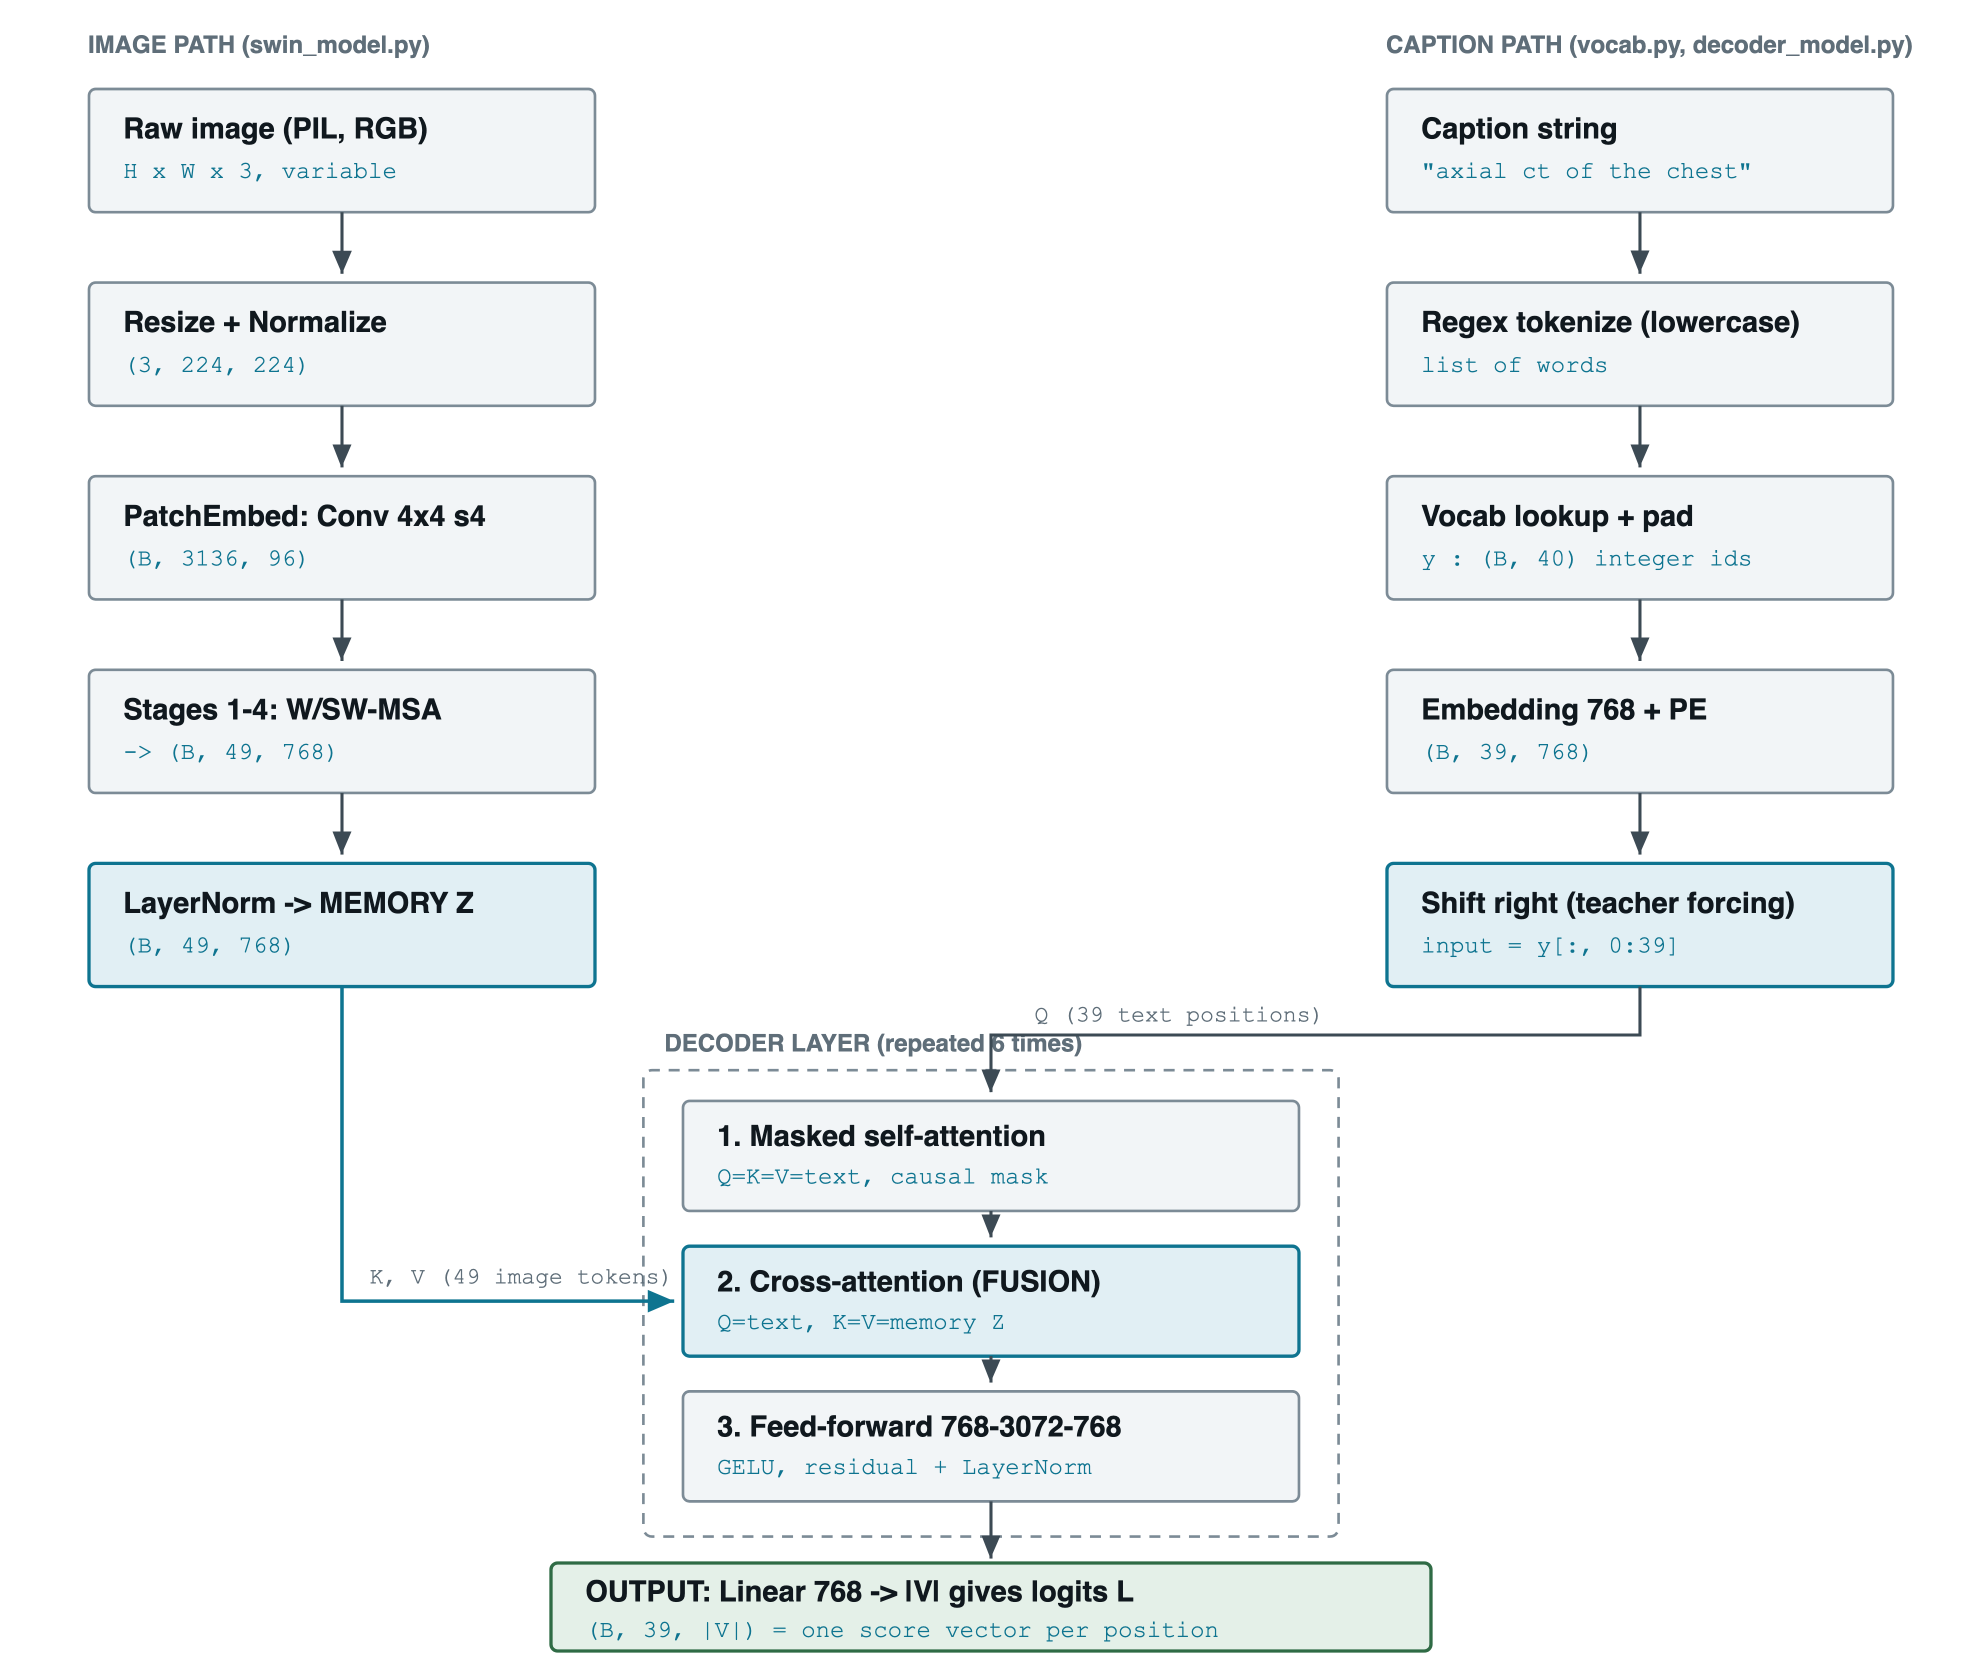
\includegraphics[width=0.95\textwidth]{figures/rId16.png}
\caption{End-to-end architecture. The Swin encoder runs once per image and produces a fixed memory of 49 visual tokens. The decoder runs 6 identical layers, and only its cross-attention sub-layer reads that memory.}
\end{figure}

The system has two input paths that meet at exactly one place.

\begin{enumerate}
\item \textbf{Image path.} A raw image is resized to a fixed $224\times224$, normalized, split into patches, and processed by four hierarchical Swin stages. The result is the image memory $Z$ of shape $(B, 49, 768)$.
\item \textbf{Caption path.} A caption string is tokenized into words, mapped to integer ids, padded to length 40, embedded into 768 dimensions and given positional information.
\item \textbf{Fusion.} Inside each decoder layer, cross-attention lets each caption position read the image memory. This is the only connection between the two paths.
\item \textbf{Output.} A linear layer maps each decoder position to a score over the whole vocabulary.
\end{enumerate}

\section{Stage A --- Image Input and Patch Embedding}

\subsection{Preprocessing}

The image is loaded, converted to RGB, resized to a fixed square, converted to a tensor with values in $[0,1]$, and normalized per channel.

\paragraph{Equation (5.1) --- Channel normalization}
\begin{equation}
X_c = \frac{X_c^{\mathrm{raw}}/255 - \mu_c}{\sigma_c}
\end{equation}
where
\begin{itemize}[nosep]
\item $X_c$ is channel $c$ of the normalized image, $c \in \{R, G, B\}$;
\item $\mu = (0.485, 0.456, 0.406)$ are the per-channel means;
\item $\sigma = (0.229, 0.224, 0.225)$ are the per-channel standard deviations.
\end{itemize}

Resizing to $224\times224$ is unconditional and does not preserve aspect ratio. During training only, two augmentations are applied before conversion to a tensor: a random rotation of up to 5 degrees and a colour jitter of 0.1 in brightness and contrast. Validation, evaluation and inference use the deterministic transform.

\subsection{Patch embedding}

The image is divided into non-overlapping $P \times P$ patches. Each patch contains $P \times P \times 3 = 48$ raw values, which are linearly projected to 96 dimensions. This is implemented as a convolution with kernel size 4 and stride 4, which is mathematically identical to splitting and projecting.

\paragraph{Equation (5.2) --- Number of patches}
\begin{equation}
N = \left(\frac{224}{P}\right)^2 = \left(\frac{224}{4}\right)^2 = 56^2 = 3136
\end{equation}

\paragraph{Equation (5.3) --- Patch projection}
\begin{equation}
z_i^0 = \mathrm{LN}\left(W_p\, \mathrm{vec}(X_i) + b_p\right)
\end{equation}
where
\begin{itemize}[nosep]
\item $X_i$ is the $i$-th patch, a $4\times4\times3$ block of the normalized image;
\item $\mathrm{vec}(\cdot)$ flattens that block into a vector in $\mathbb{R}^{48}$;
\item $W_p \in \mathbb{R}^{96\times48}$ and $b_p \in \mathbb{R}^{96}$ are learned;
\item $\mathrm{LN}$ is layer normalization, defined in Equation~(9.3);
\item $z_i^0 \in \mathbb{R}^{96}$ is the embedded token for patch $i$.
\end{itemize}

No absolute positional encoding is added to the image tokens. The Swin encoder supplies position information through a learned relative bias inside each attention window, defined in Equation~(6.4).

\subsection{Shape trace}

\begin{center}
\begin{tabular}{@{}lll@{}}
\toprule
Step & Tensor shape & Operation \\
\midrule
Load & $H \times W \times 3$ & PIL image, converted to RGB \\
Resize & $3\times224\times224$ & fixed square \\
Normalize & $3\times224\times224$ & Equation~(5.1) \\
Batch & $32\times3\times224\times224$ & DataLoader \\
Convolve $4\times4$, stride 4 & $32\times96\times56\times56$ & patch projection \\
Flatten and transpose & $32\times3136\times96$ & token sequence \\
LayerNorm & $32\times3136\times96$ & enters Stage 1 \\
\bottomrule
\end{tabular}
\end{center}

\section{Stage B --- The Swin Encoder}
\label{sec:stageb}

\begin{figure}[htbp]
\centering
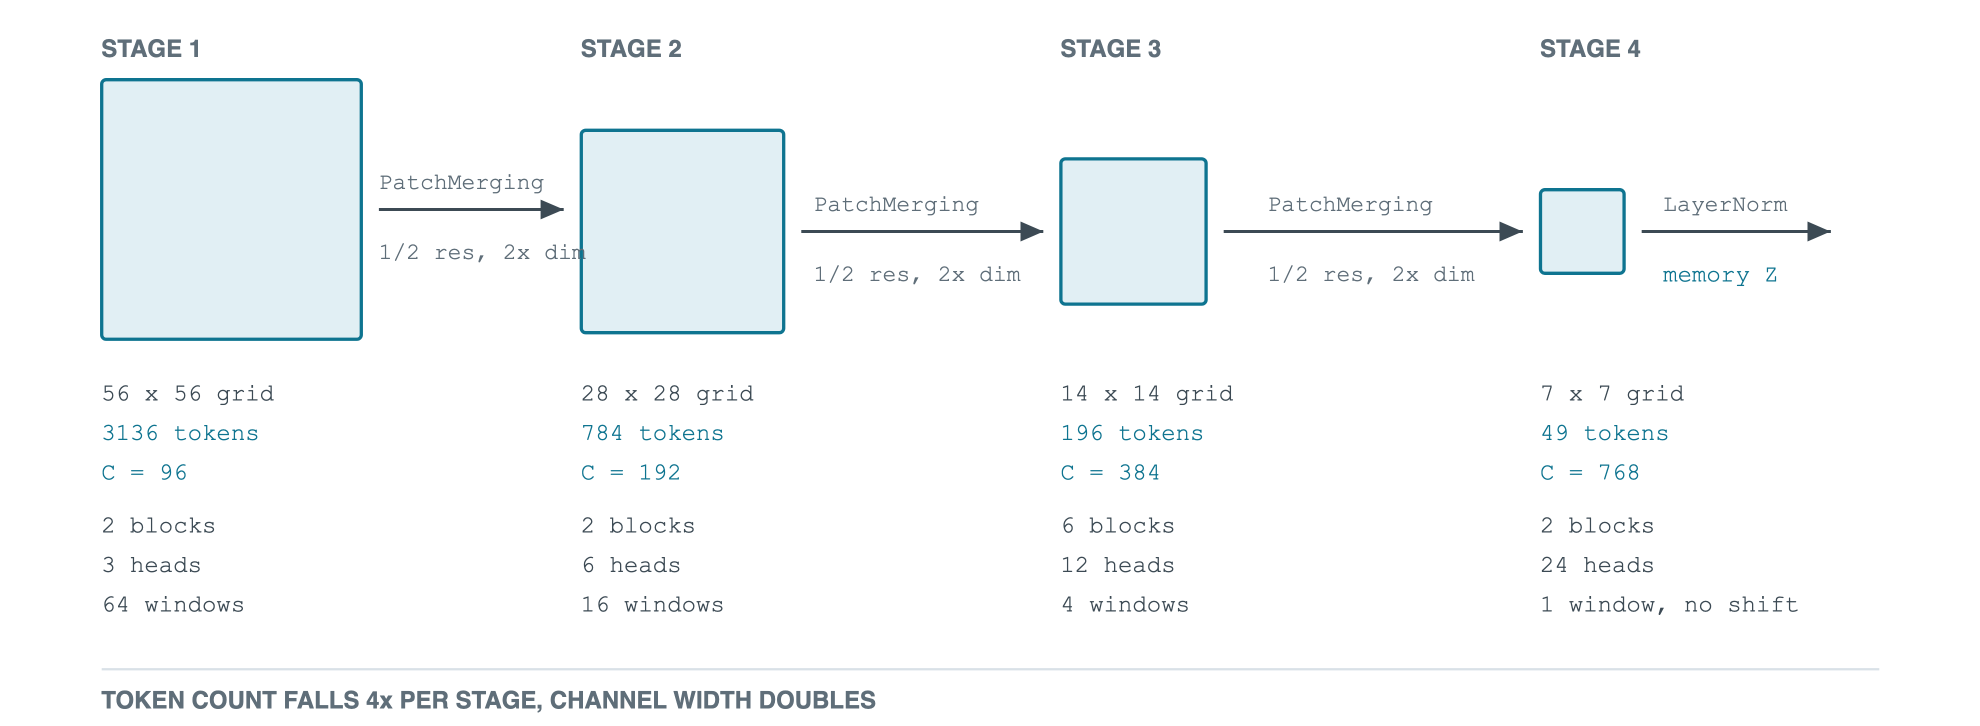
\includegraphics[width=0.85\textwidth]{figures/rId24.png}
\caption{The four-stage hierarchy. Each PatchMerging step halves the grid resolution and doubles the channel width.}
\end{figure}

\subsection{Why windows}

Computing attention over all 3136 tokens at Stage 1 is quadratic in the token count and prohibitively expensive. The Swin encoder restricts attention to non-overlapping windows of $M\times M = 7\times7 = 49$ tokens.

\paragraph{Equation (6.1) --- Cost of global attention}
\begin{equation}
\Omega(\mathrm{MSA}) = 4hwC^2 + 2(hw)^2 C
\end{equation}

\paragraph{Equation (6.2) --- Cost of window attention}
\begin{equation}
\Omega(\mathrm{W\text{-}MSA}) = 4hwC^2 + 2M^2 hw C
\end{equation}
where $h$ and $w$ are the height and width of the token grid, so $hw$ is the total token count, and $C$ is the channel width.

At Stage 1, with $hw = 3136$ and $C = 96$, the attention term falls from $2 \times 3136^2 \times 96 \approx 1.89\times10^9$ to $2 \times 49 \times 3136 \times 96 \approx 2.95\times10^7$. This is a reduction of 64 times, which is exactly the number of windows.

\subsection{Window self-attention}

\begin{figure}[htbp]
\centering
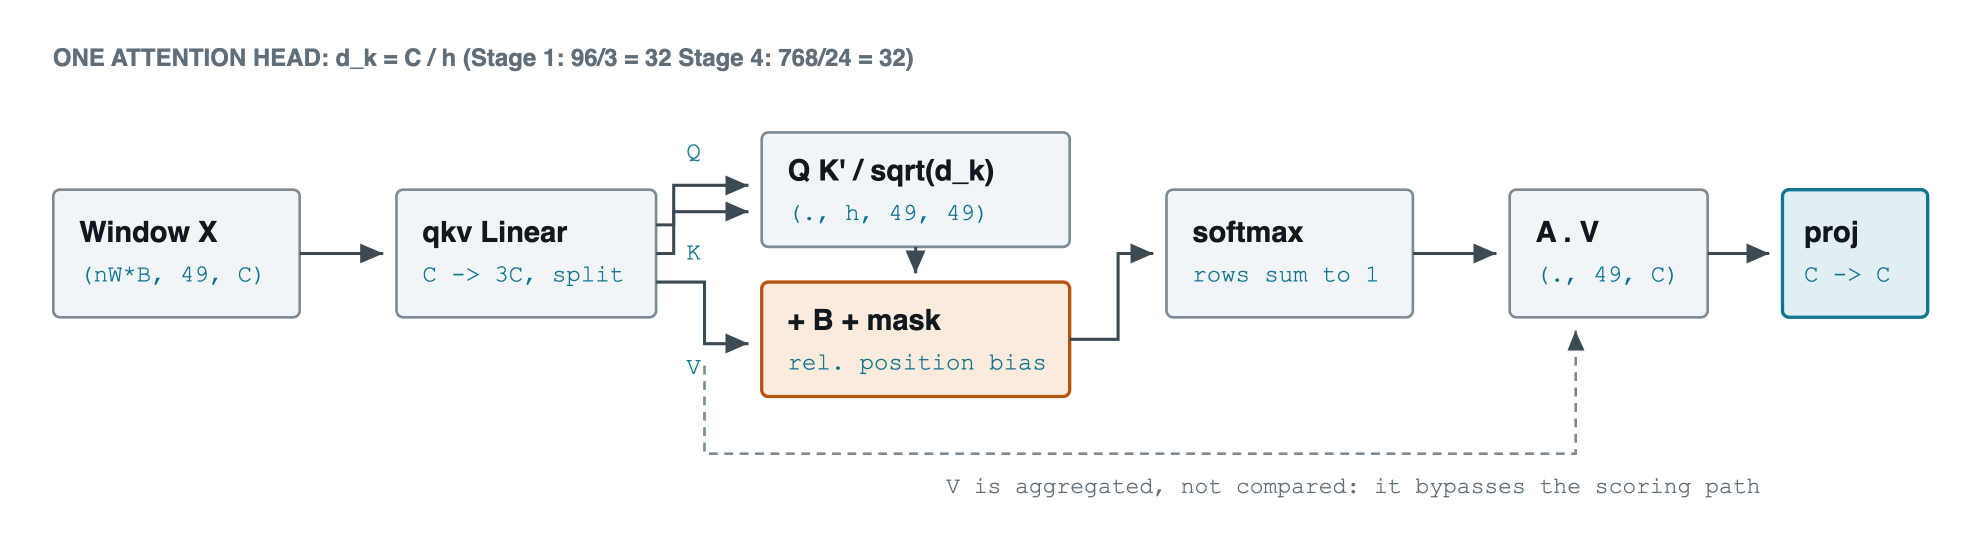
\includegraphics[width=0.7\textwidth]{figures/rId28.png}
\caption{Data flow inside one attention head. The value matrix $V$ is aggregated, not compared, so it bypasses the scoring path.}
\end{figure}

\paragraph{Equation (6.3) --- Scaled dot-product attention (the core equation)}
\begin{equation}
\mathrm{Attention}(Q,K,V) = \mathrm{softmax}\!\left(\frac{QK^\top}{\sqrt{d_k}} + \Psi\right) V
\end{equation}
where
\begin{itemize}[nosep]
\item $Q \in \mathbb{R}^{M^2 \times d_k}$ is the query matrix: what each token is looking for;
\item $K \in \mathbb{R}^{M^2 \times d_k}$ is the key matrix: what each token offers;
\item $V \in \mathbb{R}^{M^2 \times d_k}$ is the value matrix: the content each token contributes;
\item $QK^\top \in \mathbb{R}^{M^2 \times M^2}$ holds the similarity of every token pair inside the window;
\item $\sqrt{d_k}$ is a scaling factor that keeps the dot products from growing with dimension, which would otherwise push the softmax into a saturated region with vanishing gradients;
\item $\Psi$ is the relative position bias of Equation~(6.4);
\item $\mathrm{softmax}$ is applied along the last axis, so each row becomes a probability distribution over the 49 tokens of the window.
\end{itemize}

$Q$, $K$ and $V$ are produced from the window tokens $x$ by three learned linear maps, computed as a single fused projection:
\begin{equation}
Q = xW_Q, \qquad K = xW_K, \qquad V = xW_V
\end{equation}
The implementation scales $Q$ before the matrix product rather than dividing afterwards, which is algebraically identical and numerically safer.

\paragraph{Equation (6.4) --- Relative position bias}
\begin{equation}
\Psi_{ij} = \widehat{\Psi}\left[(\Delta y + M - 1)(2M-1) + (\Delta x + M - 1)\right]
\end{equation}
where
\begin{itemize}[nosep]
\item $\Delta y = y_i - y_j$ and $\Delta x = x_i - x_j$ are the row and column offsets between tokens $i$ and $j$ inside the window, each in the range $[-6, 6]$;
\item $\widehat{\Psi} \in \mathbb{R}^{169 \times h}$ is a learned lookup table with $(2M-1)^2 = 169$ entries per head, initialised from a truncated normal distribution with standard deviation 0.02;
\item the bracketed expression converts the two-dimensional offset into a single table index.
\end{itemize}

This term is what tells the model that two patches are neighbours rather than distant, and it replaces absolute positional encoding entirely on the image side.

\subsection{Shifted windows}

\begin{figure}[htbp]
\centering
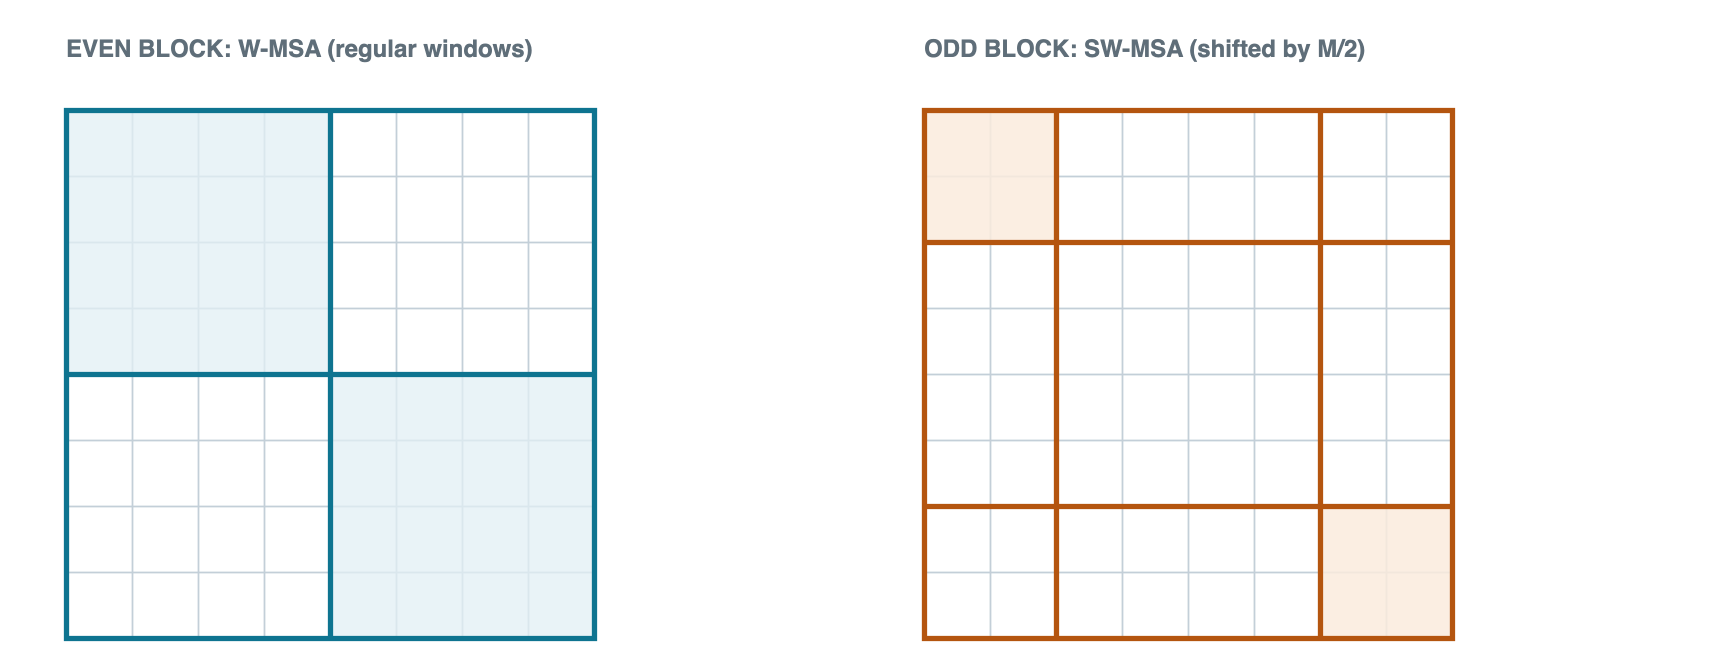
\includegraphics[width=0.6\textwidth]{figures/rId32.png}
\caption{Regular versus shifted window partition, illustrated with $M=4$ on an $8\times8$ grid for legibility. The implementation uses $M=7$ and $s=3$.}
\end{figure}

With fixed windows, tokens in different windows can never exchange information. Swin solves this by shifting the window grid in every second block, so window boundaries fall in different places.

\paragraph{Equation (6.5) --- Cyclic shift}
\begin{equation}
\tilde{z} = \mathrm{roll}(z, (-s, -s)), \qquad s = M/2 = 3
\end{equation}

The shift wraps tokens around the edges of the feature map, which places spatially distant tokens in the same window. Those pairs must not attend to each other, so an additive mask removes them.

\paragraph{Equation (6.6) --- Shifted-window mask}
\begin{equation}
\Phi_{ij} =
\begin{cases}
0 & \text{if } r(i) = r(j) \\
-100 & \text{if } r(i) \neq r(j)
\end{cases}
\end{equation}
where $r(i)$ is the index of the contiguous region that token $i$ belonged to before the shift. The mask is added to the attention scores \textbf{before} the softmax, so $e^{-100} \approx 0$ and the pair receives effectively zero weight.

The constant $-100$ is used instead of $-\infty$ because a softmax over $-\infty$ can produce NaN values on the PyTorch MPS backend. The same convention is reused in the decoder.

\subsection{The Swin block}

Blocks alternate by index parity: even-indexed blocks use regular windows (W-MSA), odd-indexed blocks use shifted windows (SW-MSA).

\paragraph{Equation (6.7) --- Swin block pair}
\begin{align}
\hat{z}^l &= \mathrm{W\text{-}MSA}(\mathrm{LN}(z^{l-1})) + z^{l-1} \\
z^l &= \mathrm{MLP}(\mathrm{LN}(\hat{z}^l)) + \hat{z}^l \\
\hat{z}^{l+1} &= \mathrm{SW\text{-}MSA}(\mathrm{LN}(z^l)) + z^l \\
z^{l+1} &= \mathrm{MLP}(\mathrm{LN}(\hat{z}^{l+1})) + \hat{z}^{l+1}
\end{align}

Each sub-layer is preceded by layer normalization and wrapped in a residual connection. The MLP has one hidden layer of width $4C$ with a GELU activation.

\subsection{Patch merging}

\paragraph{Equation (6.8) --- Patch merging}
\begin{equation}
z' = W_r\, \mathrm{LN}\left(\left[\, z_{2i,2j} \,\|\, z_{2i+1,2j} \,\|\, z_{2i,2j+1} \,\|\, z_{2i+1,2j+1} \,\right]\right)
\end{equation}
where
\begin{itemize}[nosep]
\item $\|$ denotes concatenation along the channel axis, producing a vector of width $4C$;
\item the four terms are the tokens of one $2\times2$ neighbourhood in the grid;
\item $W_r \in \mathbb{R}^{2C\times4C}$ is a learned projection with no bias.
\end{itemize}

The result halves each spatial side and doubles the channel width. It is applied after Stages 1, 2 and 3.

\subsection{Stage configuration}

\begin{center}
\begin{tabular}{@{}lccccccc@{}}
\toprule
Stage & Blocks & Heads $h$ & Grid & Tokens & $C$ & $d_k$ & Windows \\
\midrule
1 & 2 & 3  & $56\times56$ & 3136 & 96  & 32 & 64 \\
2 & 2 & 6  & $28\times28$ & 784  & 192 & 32 & 16 \\
3 & 6 & 12 & $14\times14$ & 196  & 384 & 32 & 4  \\
4 & 2 & 24 & $7\times7$   & 49   & 768 & 32 & 1  \\
\bottomrule
\end{tabular}
\end{center}

The head dimension $d_k$ remains 32 at every stage, because the head count doubles whenever the channel width doubles.

\textbf{Note on Stage 4.} Its grid is $7\times7$, which equals the window size $M=7$. The implementation detects that the feature map is not larger than one window and forces the shift to zero. Stage 4 therefore performs unshifted attention over a single window containing all 49 tokens, which is equivalent to global attention at that resolution.

A final layer normalization produces the image memory:
\begin{equation}
Z \in \mathbb{R}^{B \times 49 \times 768}
\end{equation}

\section{Stage C --- Caption Tokenization and Embedding}

\subsection{Tokenization}

Tokenization is word-level and implemented with a regular expression and a frequency counter. There is no sub-word or byte-pair encoding.

\paragraph{Equation (7.1) --- Tokenizer}
\begin{equation}
\mathrm{tok}(S) = \mathrm{split}\bigl(\mathrm{collapse}\bigl(\mathrm{strip}\bigl(\mathrm{lower}(S)\bigr)\bigr)\bigr)
\end{equation}
where the four operations, applied in order, are:
\begin{enumerate}[nosep]
\item \textbf{lower} --- convert the caption string $S$ to lowercase;
\item \textbf{strip} --- replace every character that is not a letter, digit or whitespace with a space, implemented as the substitution \code{[\^{}a-z0-9\textbackslash s]} $\to$ space;
\item \textbf{collapse} --- replace runs of consecutive whitespace with a single space and trim the ends;
\item \textbf{split} --- split on single spaces to yield the word list.
\end{enumerate}

\subsection{Vocabulary construction}

\paragraph{Equation (7.2) --- Vocabulary}
\begin{equation}
V = \{\texttt{<pad>}, \texttt{<sos>}, \texttt{<eos>}, \texttt{<unk>}\} \cup \{\, w : \mathrm{count}(w) \ge 2 \,\}
\end{equation}
where $\mathrm{count}(w)$ is the number of occurrences of word $w$ across all training captions. Words occurring only once are excluded and later map to \code{<unk>}. The four special tokens take ids 0 to 3; the remaining words are sorted alphabetically.

Vocabulary size depends directly on how many captions are used:

\begin{center}
\begin{tabular}{@{}lc@{}}
\toprule
Training captions & $|V|$ \\
\midrule
2,000  & 2,682 \\
5,000  & 4,493 \\
10,000 & 6,439 \\
15,000 & 7,886 \\
\bottomrule
\end{tabular}
\end{center}

\subsection{Encoding a caption}

\paragraph{Equation (7.3) --- Token id sequence}
\begin{equation}
y = [\, \texttt{<sos>}, w_1, \ldots, w_m, \texttt{<eos>}, \texttt{<pad>}, \ldots \,] \in \mathbb{N}^T
\end{equation}
where $m \le T-2 = 38$ content words are kept, any word not in $V$ is replaced by \code{<unk>}, longer captions are truncated, and shorter ones are right-padded with \code{<pad>} up to $T=40$.

\subsection{Embedding and position}

\paragraph{Equation (7.4) --- Token embedding}
\begin{equation}
x_t^{(0)} = \mathrm{Dropout}_{0.1}\bigl(E[y_t] + \mathrm{PE}_t\bigr)
\end{equation}
where $E \in \mathbb{R}^{|V|\times768}$ is a learned embedding matrix and $E[y_t]$ selects the row for token id $y_t$.

\paragraph{Equation (7.5) --- Sinusoidal positional encoding}
\begin{equation}
\mathrm{PE}_{(t,2i)} = \sin\!\left(\frac{t}{10000^{2i/d}}\right), \qquad
\mathrm{PE}_{(t,2i+1)} = \cos\!\left(\frac{t}{10000^{2i/d}}\right)
\end{equation}
where $t$ is the position, $i$ indexes the dimension pair, and $d=768$. This table is fixed, not learned, and carries no gradient. It gives the model a notion of word order, which attention alone does not provide.

\section{Stage D --- Caption Masking and Cross-Attention Fusion}
\label{sec:staged}

\subsection{Teacher forcing and the input/target split}

During training the model is shown the correct caption but must always predict one position ahead. The padded caption is split into two sequences offset by one position.

\paragraph{Equation (8.1) --- Input and target}
\begin{equation}
\mathrm{input} = y[0:T-1], \qquad \mathrm{target} = y[1:T], \qquad T' = 39
\end{equation}

So the input begins with \code{<sos>} and excludes the last token; the target excludes \code{<sos>} and is the word the model must produce at each position. This is called \textbf{teacher forcing}: the model receives the ground-truth prefix rather than its own previous predictions.

\subsection{The causal mask}

\begin{figure}[htbp]
\centering
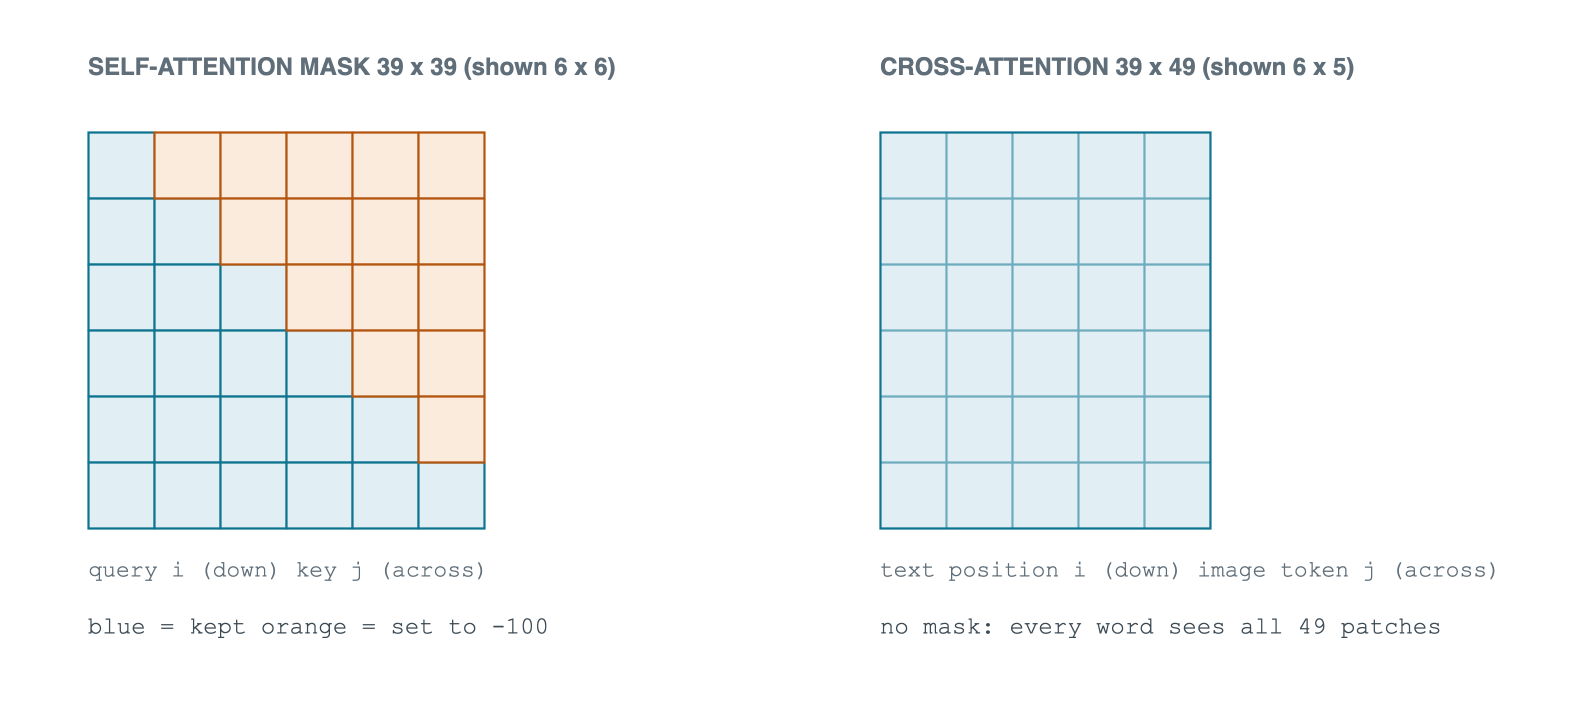
\includegraphics[width=0.55\textwidth]{figures/rId46.png}
\caption{Self-attention is masked to a lower-triangular pattern; cross-attention is unmasked and fully dense.}
\end{figure}

\paragraph{Equation (8.2) --- Causal mask}
\begin{equation}
\Gamma = \mathrm{tril}(\mathbf{1}_{T'\times T'}), \qquad
\Gamma_{ij} =
\begin{cases}
1 & j \le i \\
0 & j > i
\end{cases}
\end{equation}

\paragraph{Equation (8.3) --- Applying the mask}
\begin{equation}
\tilde{A}_{ij} =
\begin{cases}
A_{ij} & \Gamma_{ij} = 1 \\
-100 & \Gamma_{ij} = 0
\end{cases}
\end{equation}
where $A_{ij}$ is the raw attention score before softmax. Position $i$ may therefore attend only to positions $j \le i$, that is, to itself and to the past.

\textbf{Why this is required.} Without the mask, the representation at position $t$ would incorporate the words at positions $t+1$ and beyond. The model would learn to copy the answer from its own input and would fail completely at generation time, when future words do not exist.

\subsection{Cross-attention: the fusion point}

Cross-attention differs from self-attention in exactly one respect: the queries come from the caption, while the keys and values come from the image.

\paragraph{Equation (8.4) --- Cross-attention projections}
\begin{equation}
Q = xW_Q, \qquad K = ZW_K, \qquad V = ZW_V
\end{equation}
where $x \in \mathbb{R}^{B\times39\times768}$ is the decoder hidden state and $Z \in \mathbb{R}^{B\times49\times768}$ is the image memory. Therefore $Q$ has 39 rows and $K, V$ have 49 rows.

\paragraph{Equation (8.5) --- Cross-attention}
\begin{equation}
C = \mathrm{softmax}\!\left(\frac{QK^\top}{\sqrt{d_k}}\right)V, \qquad d_k = \frac{768}{8} = 96
\end{equation}

The score matrix $QK^\top$ has shape $(B, 8, 39, 49)$. Row $t$ of this matrix, after softmax, is a probability distribution over the 49 image patches, and answers the question: \emph{which regions of the image does word $t$ look at?}

\textbf{No mask is applied here.} The image is fully observable at every position, past and future alike, because the image is not something the model has to predict. Masking is a property of the caption sequence only.

\textbf{Why this connection is critical.} Cross-attention is the only path by which gradient reaches the Swin encoder. During backpropagation, the derivative of the loss with respect to $Z$ arrives exclusively through $W_K$ and $W_V$ in the six decoder layers. If these attention maps collapse to a uniform distribution, the encoder receives almost no learning signal and the system degenerates into a language model that ignores the image.

\section{Stage E --- The Decoder and Its Output}
\label{sec:stagee}

\subsection{Structure of one decoder layer}

\begin{figure}[htbp]
\centering
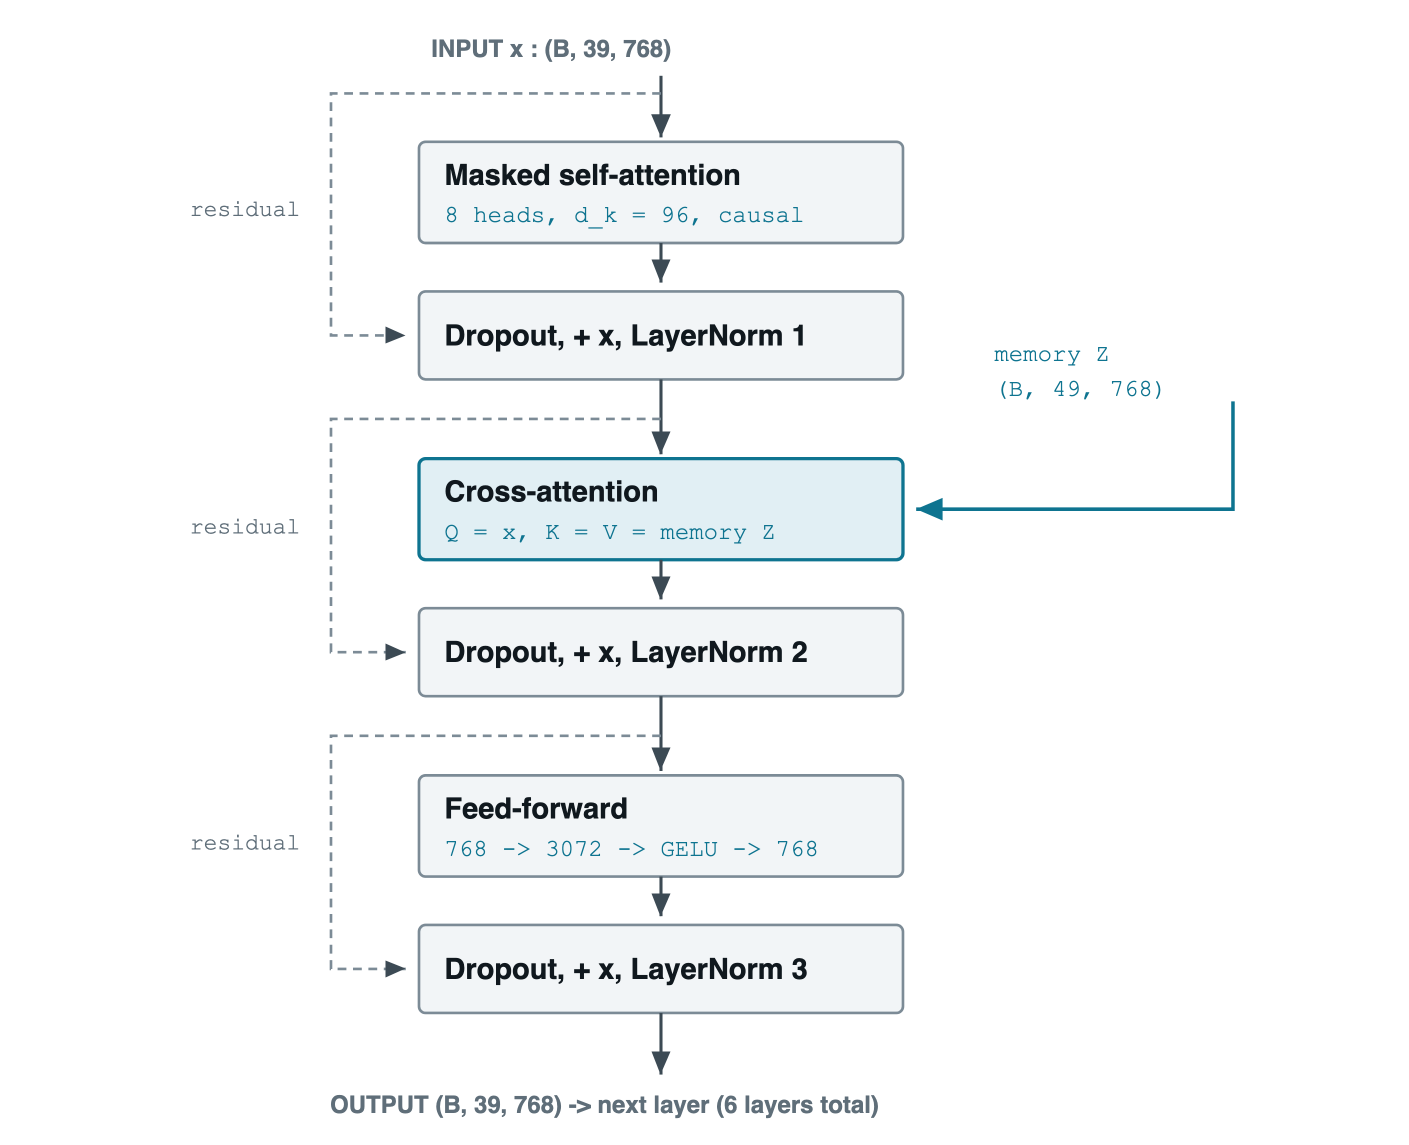
\includegraphics[width=0.65\textwidth]{figures/rId52.png}
\caption{One decoder layer. Normalization is applied after the residual sum in each of the three sub-layers.}
\end{figure}

\paragraph{Equation (9.1) --- Decoder layer}
\begin{align}
x &\leftarrow \mathrm{LN}_1\bigl(x + \mathrm{Drop}(\mathrm{SelfAttn}(x,x,x;\Gamma))\bigr) \\
x &\leftarrow \mathrm{LN}_2\bigl(x + \mathrm{Drop}(\mathrm{CrossAttn}(x,Z,Z))\bigr) \\
x &\leftarrow \mathrm{LN}_3\bigl(x + \mathrm{Drop}(W_2\,\mathrm{GELU}(W_1 x + b_1) + b_2)\bigr)
\end{align}
where $\mathrm{Drop}$ is dropout with probability 0.1, and the feed-forward network expands $768 \to 3072 \to 768$.

\paragraph{Equation (9.2) --- Multi-head attention}
\begin{equation}
\mathrm{MultiHead}(Q,K,V) = \left[\,\mathrm{head}_1 \,\|\, \cdots \,\|\, \mathrm{head}_8\,\right] W_O
\end{equation}
Each head operates in an independent 96-dimensional subspace; the eight outputs are concatenated and projected back to 768 dimensions by $W_O$.

\paragraph{Equation (9.3) --- Layer normalization}
\begin{equation}
\mathrm{LN}(x) = \gamma \odot \frac{x - \mu}{\sqrt{\sigma^2 + \epsilon}} + \beta
\end{equation}
where $\mu$ and $\sigma^2$ are the mean and variance computed across the feature axis of a single token, $\gamma$ and $\beta$ are learned scale and shift vectors, and $\odot$ is element-wise multiplication.

\paragraph{Equation (9.4) --- GELU activation}
\begin{equation}
\mathrm{GELU}(x) = x \cdot \Phi_{\mathcal{N}}(x)
\end{equation}
where $\Phi_{\mathcal{N}}$ is the cumulative distribution function of the standard normal distribution.

Six such layers are stacked. Layer $l$ receives the output of layer $l-1$; all six read the same image memory $Z$.

\subsection{What the decoder output actually is}

\begin{figure}[htbp]
\centering
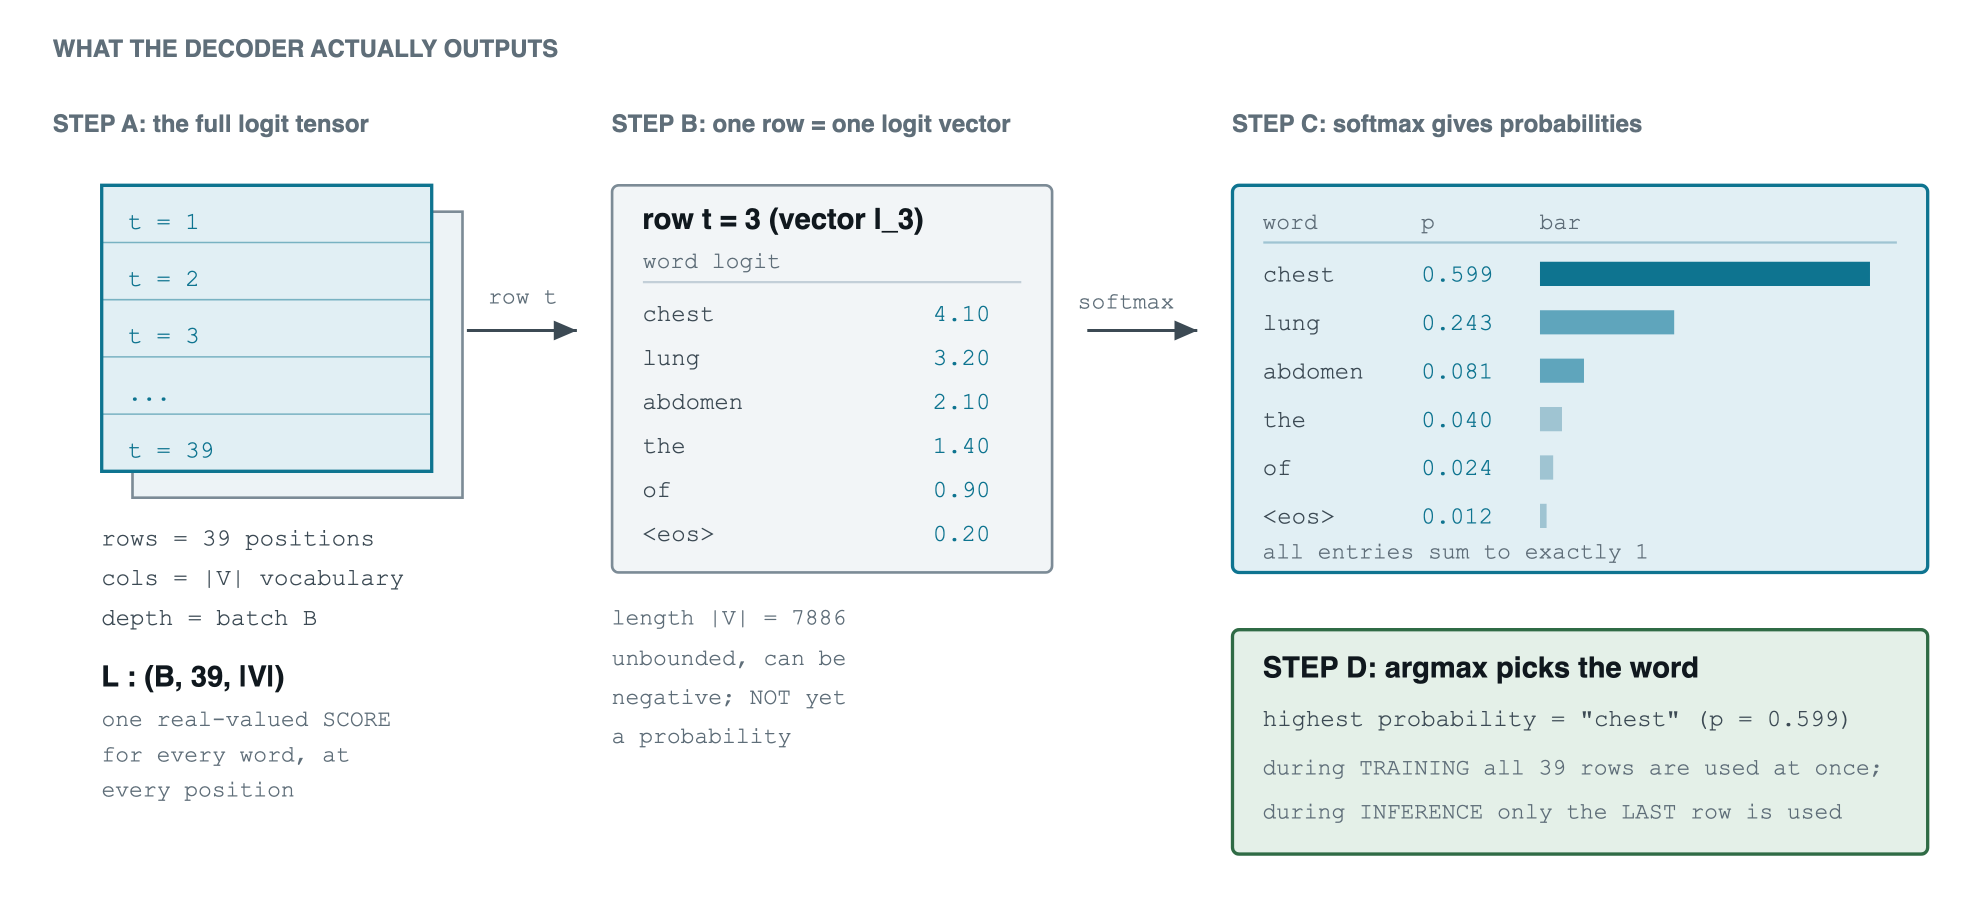
\includegraphics[width=0.75\textwidth]{figures/rId56.png}
\caption{The decoder output explained in four steps: the full logit tensor, one row of it, the softmax that turns it into probabilities, and the argmax that selects a word.}
\end{figure}

This subsection answers the question directly: \textbf{the decoder does not output words. It outputs numbers, one per vocabulary entry, per position.}

\paragraph{Equation (9.5) --- Output projection}
\begin{equation}
\ell_t = W_O' x_t^{(6)} + b_O', \qquad \ell_t \in \mathbb{R}^{|V|}
\end{equation}
where $x_t^{(6)} \in \mathbb{R}^{768}$ is the hidden state at position $t$ after all six layers, and $W_O' \in \mathbb{R}^{|V|\times768}$ is the output projection.

Stacking over positions and batch gives the full output tensor:
\begin{equation}
L \in \mathbb{R}^{B \times 39 \times |V|}
\end{equation}

The three axes mean:
\begin{itemize}[nosep]
\item axis 1 ($B=32$): which image in the mini-batch;
\item axis 2 ($T'=39$): which position in the caption;
\item axis 3 ($|V|=7886$): which vocabulary word.
\end{itemize}

A single entry $L[b,t,w]$ is therefore the score that image $b$ assigns to word $w$ being the next word at position $t$. These scores are called \textbf{logits}. They are unbounded real numbers, may be negative, and are not probabilities.

\paragraph{Equation (9.6) --- Softmax converts logits into probabilities}
\begin{equation}
p_t(w) = \frac{\exp(\ell_t(w))}{\sum_{w' \in V} \exp(\ell_t(w'))}
\end{equation}
After this operation every entry lies in $[0,1]$ and the entries at a given position sum to exactly 1, so $p_t$ is a genuine probability distribution over the vocabulary.

How the output is used differs between the two phases:

\begin{center}
\begin{tabular}{@{}lL{3.2cm}L{7cm}@{}}
\toprule
Phase & Rows of $L$ used & What happens to them \\
\midrule
Training & All 39 rows at once & Every row is compared with its ground-truth target word by the loss of Equation~(10.1). One forward pass supplies 39 training signals per caption. \\[4pt]
Inference & Only the last row & Rows before the last are recomputed but discarded, because only the newest position predicts a genuinely unknown word. See Section~\ref{sec:inference}. \\
\bottomrule
\end{tabular}
\end{center}

\subsection{Parameter count}

\begin{center}
\begin{tabular}{@{}lll@{}}
\toprule
Component & Configuration & Parameters at $|V|=7{,}886$ \\
\midrule
Token embedding & $7886\times768$ & $\approx 6.06$ M \\
Self-attention, per layer & $4\times768^2$ & $\approx 2.36$ M \\
Cross-attention, per layer & $4\times768^2$ & $\approx 2.36$ M \\
Feed-forward, per layer & $2\times768\times3072$ & $\approx 4.72$ M \\
Six decoder layers & --- & $\approx 56.6$ M \\
Output projection & $768\times7886$ & $\approx 6.06$ M \\
\bottomrule
\end{tabular}
\end{center}

\section{Training and Weight Adjustment}
\label{sec:training}

\begin{figure}[htbp]
\centering
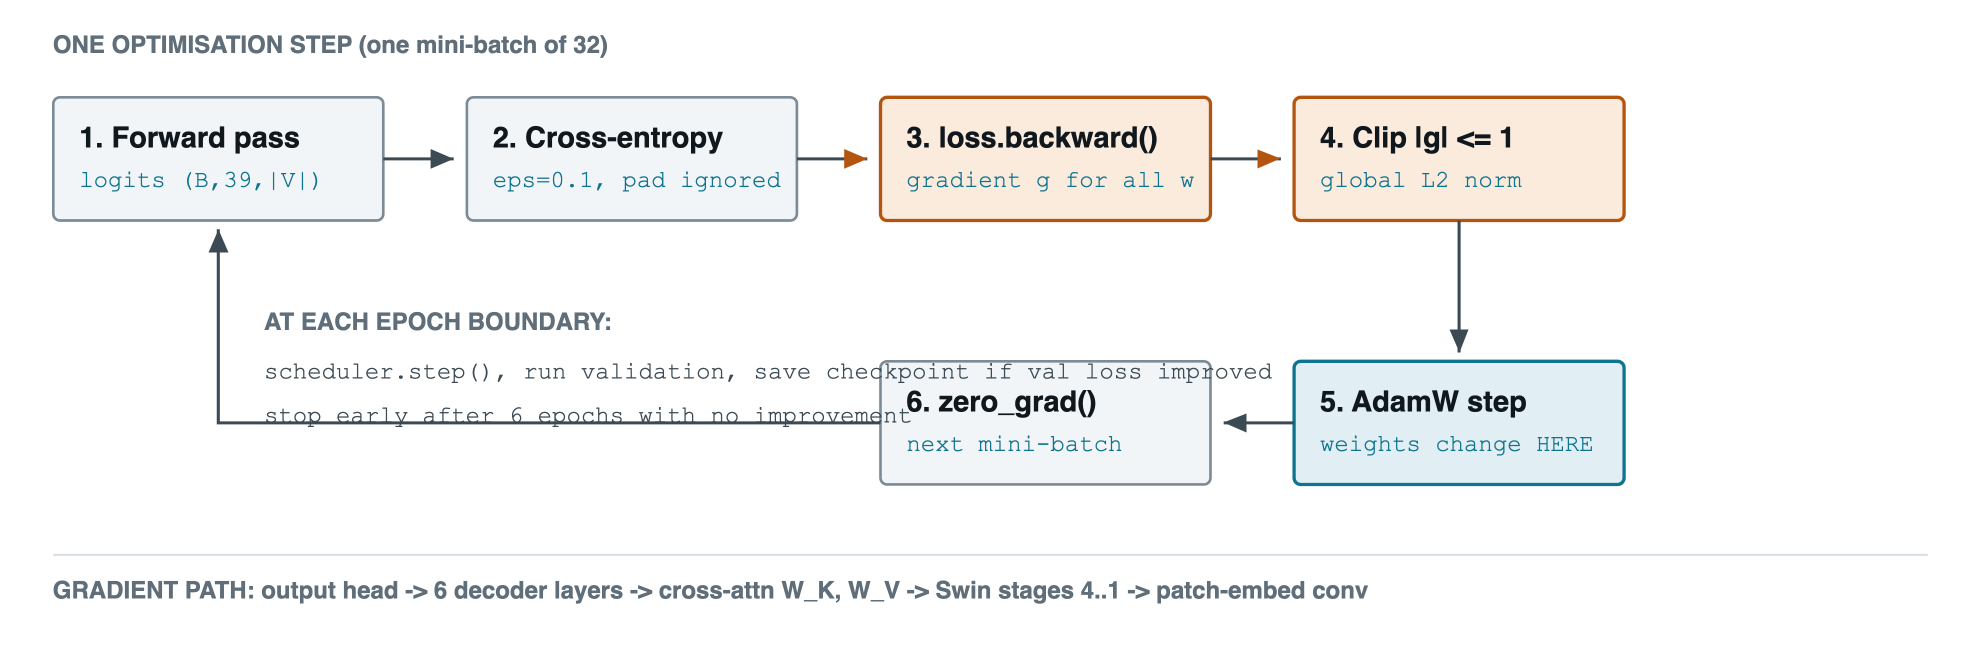
\includegraphics[width=0.7\textwidth]{figures/rId62.png}
\caption{One optimisation step. The weights change only at step 5.}
\end{figure}

\subsection{The objective}

\paragraph{Equation (10.1) --- Label-smoothed cross-entropy loss}
\begin{equation}
J = -\frac{1}{|S|} \sum_{t \in S} \sum_{w \in V} q_t(w) \log p_t(w)
\end{equation}
where
\begin{itemize}[nosep]
\item $S = \{\, t : \mathrm{target}_t \neq \texttt{<pad>} \,\}$ is the set of non-padding positions, so padding never contributes to the loss;
\item $p_t(w)$ is the model probability from Equation~(9.6);
\item $q_t(w)$ is the smoothed target distribution below.
\end{itemize}

\paragraph{Equation (10.2) --- Label smoothing}
\begin{equation}
q_t(w) = (1-\varepsilon)\,\mathbf{1}[w = y_t] + \frac{\varepsilon}{|V|}, \qquad \varepsilon = 0.1
\end{equation}
where $\mathbf{1}[\cdot]$ is the indicator function, equal to 1 when its condition holds and 0 otherwise. The target is therefore never a hard one-hot vector: the correct word receives 0.9 plus a small share, and every other word receives $\varepsilon/|V|$. This caps how large the model can profitably drive its logits and prevents over-confidence on a small medical vocabulary.

\subsection{How the weights are adjusted}

This subsection specifies the weight update precisely. The procedure repeats for every mini-batch.

\textbf{Step 1 --- Compute the gradient.} Backpropagation applies the chain rule in reverse through the computation graph to obtain

\paragraph{Equation (10.3) --- Gradient}
\begin{equation}
g_k = \nabla_\theta J
\end{equation}
which is the derivative of the loss with respect to every trainable weight, evaluated at optimizer step $k$. The gradient traverses, in order: the output projection, the six decoder layers, the cross-attention key and value projections, the four Swin stages in reverse, and finally the patch-embedding convolution. \textbf{Both encoder and decoder are trained jointly}, from random initialisation, with no frozen components.

\textbf{Step 2 --- Clip the gradient.}

\paragraph{Equation (10.4) --- Global norm clipping}
\begin{equation}
g_k \leftarrow g_k \cdot \min\!\left(1, \frac{1}{\|g_k\|_2}\right)
\end{equation}
where $\|g_k\|_2$ is the L2 norm computed over all parameters jointly. If the norm exceeds 1, the whole gradient is rescaled to norm 1. This bounds the damage from an occasional unstable batch.

\textbf{Step 3 --- Update the moment estimates.} AdamW maintains a running average of the gradient and of its square.

\paragraph{Equation (10.5) --- First moment (mean of gradients)}
\begin{equation}
m_k = \beta_1 m_{k-1} + (1-\beta_1) g_k, \qquad \beta_1 = 0.9
\end{equation}

\paragraph{Equation (10.6) --- Second moment (mean of squared gradients)}
\begin{equation}
v_k = \beta_2 v_{k-1} + (1-\beta_2) g_k^2, \qquad \beta_2 = 0.999
\end{equation}

\paragraph{Equation (10.7) --- Bias correction}
\begin{equation}
\hat{m}_k = \frac{m_k}{1-\beta_1^k}, \qquad \hat{v}_k = \frac{v_k}{1-\beta_2^k}
\end{equation}
Bias correction is needed because $m$ and $v$ are initialised at zero and would otherwise be biased towards zero during the first steps.

\textbf{Step 4 --- Apply the update.} This is the point at which the weights change.

\paragraph{Equation (10.8) --- AdamW update rule}
\begin{equation}
\theta_k = \theta_{k-1} - \eta_e \left(\frac{\hat{m}_k}{\sqrt{\hat{v}_k} + \epsilon_{\mathrm{adam}}} + \lambda \theta_{k-1}\right)
\end{equation}
where
\begin{itemize}[nosep]
\item $\theta_{k-1}$ are the weights before the step and $\theta_k$ after it;
\item $\eta_e$ is the learning rate for the current epoch, from Equation~(10.10);
\item $\hat{m}_k$ is the direction of travel, a smoothed gradient;
\item $\sqrt{\hat{v}_k}$ rescales each weight's step by the recent magnitude of its own gradient, so rarely-updated weights take larger steps than frequently-updated ones;
\item $\epsilon_{\mathrm{adam}} = 10^{-8}$ prevents division by zero;
\item $\lambda \theta_{k-1}$ is \textbf{decoupled weight decay}, which shrinks each weight towards zero in proportion to its own size. It is applied directly to the weight rather than being folded into the gradient, which is the distinguishing feature of AdamW compared with Adam.
\end{itemize}

\paragraph{Equation (10.9) --- Weight decay assignment}
\begin{equation}
\lambda =
\begin{cases}
0.05 & \text{if } \theta \text{ has more than one dimension and is not a bias table} \\
0 & \text{otherwise}
\end{cases}
\end{equation}
Parameters exempted from decay are: all LayerNorm scales and shifts, all linear biases, and the relative position bias table $\widehat{\Psi}$. The last of these is two-dimensional and so must be excluded by name rather than by shape. Decaying these distorts normalisation scale and the learned window geometry without improving generalisation.

\textbf{Step 5 --- Reset.} Gradients are zeroed before the next mini-batch, because PyTorch accumulates them by default.

\subsection{Learning rate schedule}

\paragraph{Equation (10.10) --- Warmup and cosine decay}
\begin{equation}
\eta_e = \eta_{\mathrm{peak}} \cdot
\begin{cases}
\dfrac{e+1}{5} & e < 5 \\[8pt]
\dfrac{1}{2}\left(1 + \cos\dfrac{\pi(e-5)}{55}\right) & e \ge 5
\end{cases}
\end{equation}
with $\eta_{\mathrm{peak}} = 5\times10^{-4}$. The rate rises linearly over the first five epochs, which stabilises the early steps while the moment estimates are still poor, then decays smoothly to zero over the remaining 55. The schedule advances once per epoch, not per batch.

\subsection{Validation, checkpointing and early stopping}

At the end of every epoch the model is switched to evaluation mode and the validation loss is computed under \code{torch.no\_grad()} using the \textbf{same teacher-forced objective} of Equation~(10.1). Validation does not use generation, so the training and validation numbers are directly comparable.

\begin{itemize}[nosep]
\item If the validation loss improves on the best value so far, the checkpoint is written and the patience counter resets.
\item Otherwise the patience counter increments.
\item If the counter reaches 6, training stops early.
\end{itemize}

\subsection{Hyperparameters}

\begin{center}
\begin{tabular}{@{}lll@{}}
\toprule
Hyperparameter & Value & Purpose \\
\midrule
Training samples & 15,000 & slice of the 59,958 available \\
Validation samples & 2,000 & slice of the 9,904 available \\
Batch size & 32 & fits single-GPU and MPS memory \\
Epochs & 60 & with early stopping, patience 6 \\
Peak learning rate & $5\times10^{-4}$ & 5 warmup epochs, then cosine \\
Weight decay $\lambda$ & 0.05 & multi-dimensional weights only \\
Label smoothing $\varepsilon$ & 0.1 & prevents over-confidence \\
Gradient clip & 1.0 & global L2 norm \\
Dropout & 0.1 & decoder residual branches \\
\bottomrule
\end{tabular}
\end{center}

\section{Inference --- Generating a Caption for a New Image}
\label{sec:inference}

\begin{figure}[htbp]
\centering
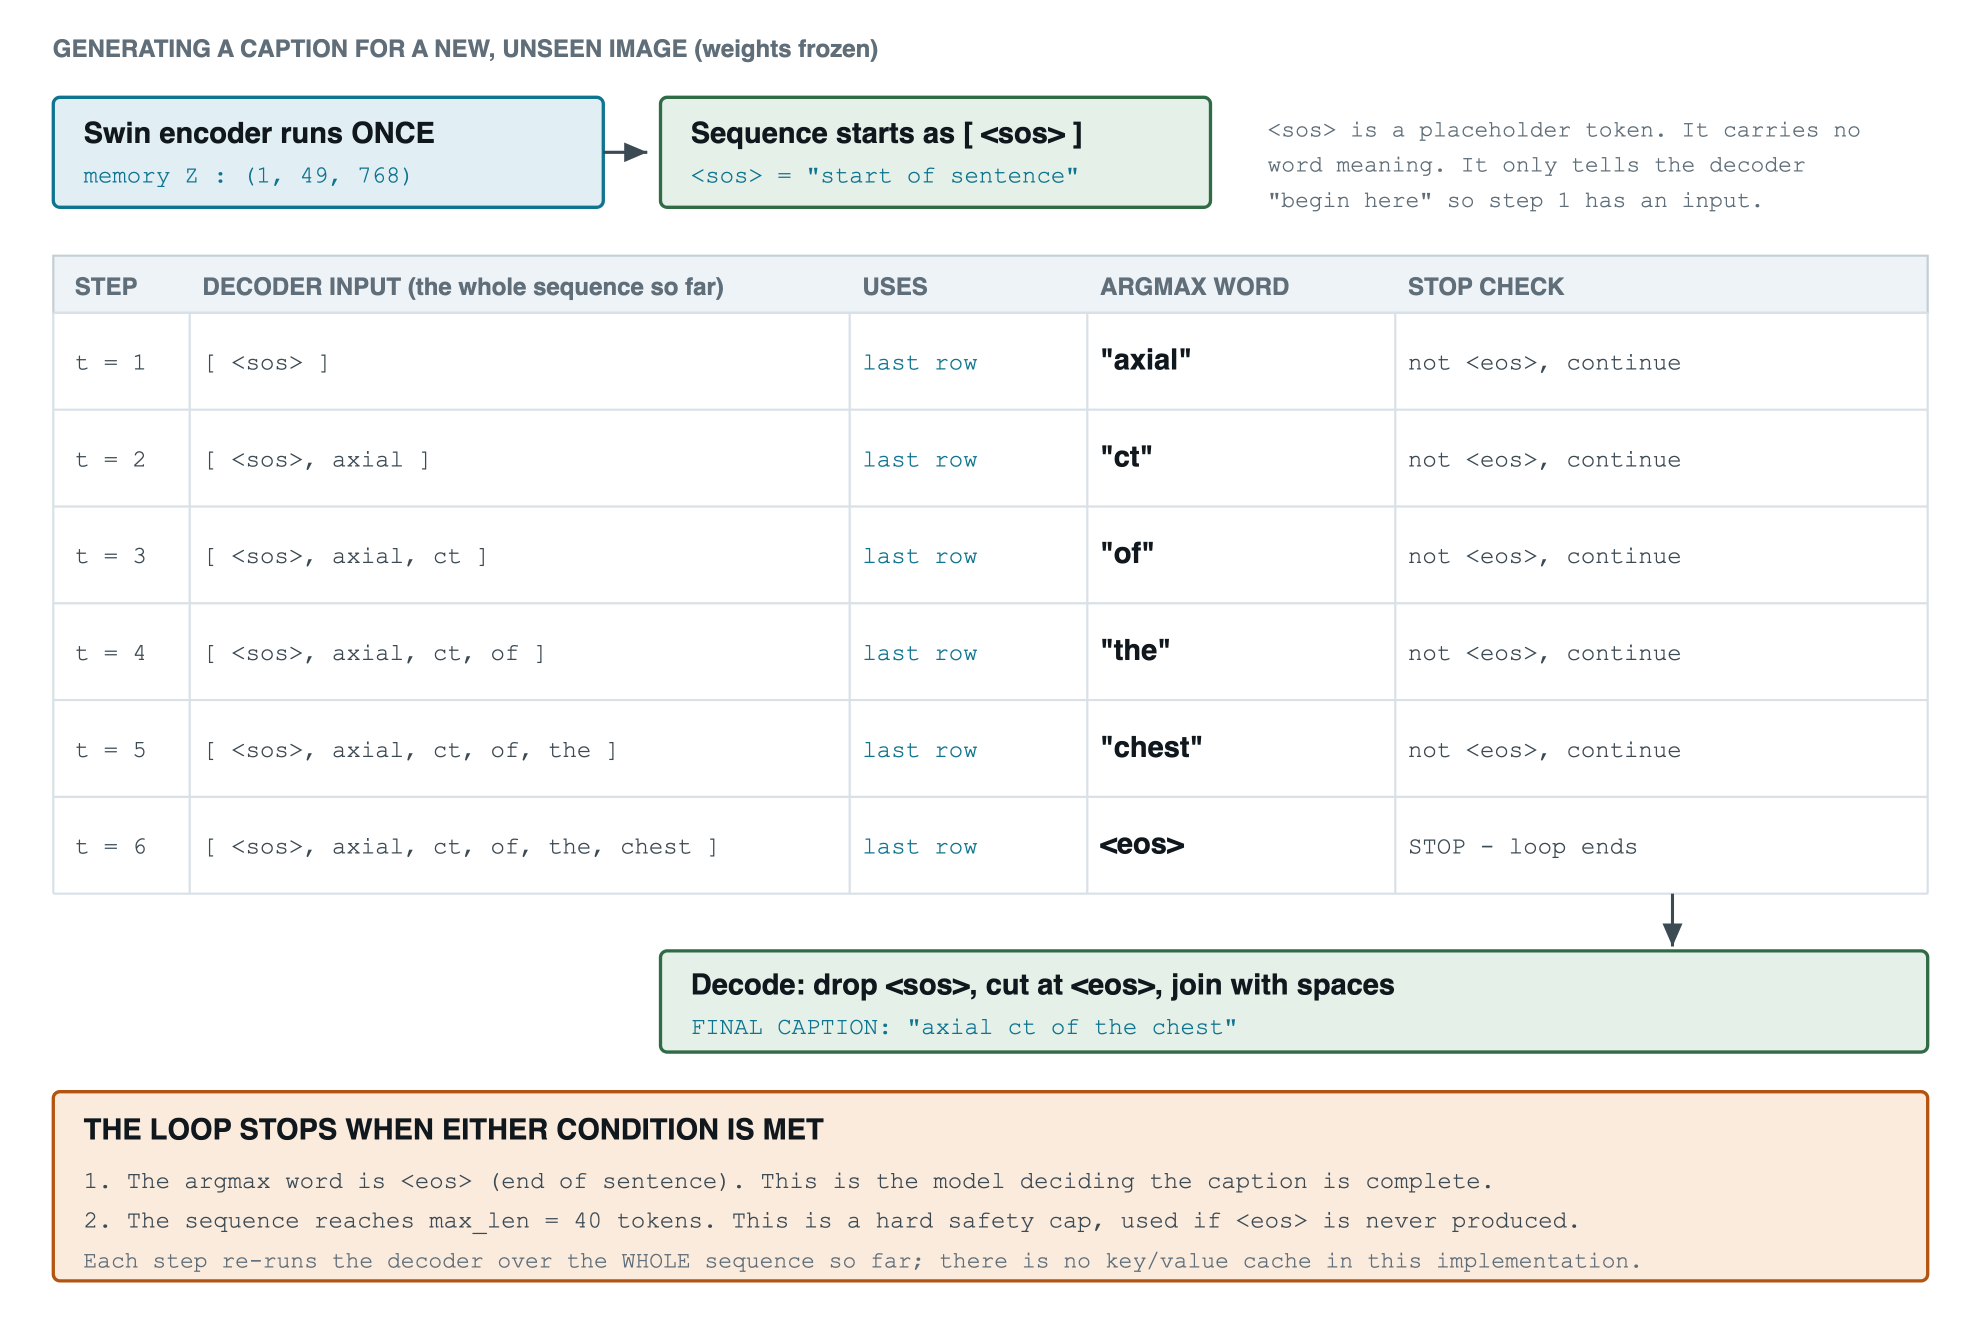
\includegraphics[width=0.75\textwidth]{figures/rId71.png}
\caption{A complete generation trace, with the two stopping conditions stated explicitly.}
\end{figure}

At inference the weights are frozen: no gradient is computed and nothing is updated. The task changes from ``score a caption I was given'' to ``build a caption one word at a time.''

\subsection{The core difficulty and how it is solved}

At training time the whole caption is available and all 39 positions are predicted in one pass. At test time no caption exists. The model must therefore construct one \textbf{autoregressively}: predict one word, append it to the sequence, and feed the extended sequence back in to predict the next word.

The sequence has to start somewhere, and this is precisely why the \code{<sos>} token exists. It is a content-free placeholder whose only role is to be the first input, so that step 1 has something to condition on.

\subsection{The procedure}

\textbf{Step 0 --- Encode the image once.}
\begin{equation}
Z = \mathrm{SwinEncoder}(X), \qquad Z \in \mathbb{R}^{1\times49\times768}
\end{equation}
The encoder is not run again. The same memory $Z$ is reused at every subsequent step.

\textbf{Step 1 --- Initialise the sequence.}
\begin{equation}
\hat{y} = [\, \texttt{<sos>} \,]
\end{equation}

\textbf{Step 2 --- Repeat until a stopping condition is met.} At step $t$, with the sequence $\hat{y}_{1:t}$ built so far:

\paragraph{Equation (11.1) --- Forward pass and last-row extraction}
\begin{equation}
\ell_t = \mathrm{Decoder}(\hat{y}_{1:t}, Z)\,[\text{last row}]
\end{equation}
The decoder returns a logit tensor of shape $(1, t, |V|)$, but only the final row is used, because that row is the prediction for the position \emph{after} the last known token. The earlier rows merely re-predict words that are already fixed.

\paragraph{Equation (11.2) --- Constraint set}
\begin{align}
D_t &= \{\hat{y}_t\} \cup \{\, w : (\hat{y}_{t-1}, \hat{y}_t, w) \text{ already occurs in } \hat{y}_{1:t} \,\} \\
A_t &= V - D_t
\end{align}
Two hard constraints are imposed by setting the corresponding logits to $-\infty$ before selection:
\begin{enumerate}[nosep]
\item \textbf{No immediate repetition.} The word just produced cannot be produced again at the next step.
\item \textbf{No repeated trigram.} If the pair $(\hat{y}_{t-1}, \hat{y}_t)$ has been followed by word $w$ earlier in the sequence, $w$ is banned now.
\end{enumerate}
These suppress the degenerate loops that purely greedy decoding falls into.

\paragraph{Equation (11.3) --- Greedy selection of the next word}
\begin{equation}
\hat{y}_{t+1} = \arg\max_{w \in A_t} \ell_t(w)
\end{equation}
The chosen word is the single highest-scoring allowed vocabulary entry. Because $\arg\max$ is unaffected by the monotone softmax transform, the implementation applies it directly to the logits and never materialises the probabilities. Conceptually, however, the selection is over $p_t$ from Equation~(9.6).

\paragraph{Equation (11.4) --- Sequence extension}
\begin{equation}
\hat{y}_{1:t+1} = [\, \hat{y}_{1:t} \,\|\, \hat{y}_{t+1} \,]
\end{equation}
The new word is appended and control returns to Equation~(11.1).

\subsection{Worked trace}

Following the generation trace, with the model producing the caption ``axial ct of the chest'':

\begin{center}
\begin{tabular}{@{}cL{5.2cm}cl@{}}
\toprule
Step $t$ & Decoder input & Selected word & Continue? \\
\midrule
1 & [\code{<sos>}] & axial & yes \\
2 & [\code{<sos>}, axial] & ct & yes \\
3 & [\code{<sos>}, axial, ct] & of & yes \\
4 & [\code{<sos>}, axial, ct, of] & the & yes \\
5 & [\code{<sos>}, axial, ct, of, the] & chest & yes \\
6 & [\code{<sos>}, axial, ct, of, the, chest] & \code{<eos>} & \textbf{no --- stop} \\
\bottomrule
\end{tabular}
\end{center}

\subsection{When generation stops}
\label{sec:inference-stop}

The loop terminates when \textbf{either} condition is satisfied:
\begin{enumerate}[nosep]
\item \textbf{The selected word is \code{<eos>}.} This is the model's own judgement that the caption is complete. It is the normal termination path, and it is learned: during training the model was always shown \code{<eos>} immediately after the last real word, so it learns to assign \code{<eos>} the highest score once the description is finished.
\item \textbf{The sequence reaches $T=40$ tokens.} This is a hard safety cap that guarantees termination if the model never emits \code{<eos>}. It is a failure-mode guard, not the intended exit.
\end{enumerate}

\subsection{Converting ids back to text}

The final id sequence is decoded by scanning left to right and:
\begin{itemize}[nosep]
\item stopping at the first \code{<eos>};
\item skipping \code{<sos>} and \code{<pad>};
\item mapping every remaining id to its word and joining with single spaces.
\end{itemize}
For the trace above this yields ``axial ct of the chest''.

\subsection{Cost and limitations}

One caption requires one encoder pass and up to 39 decoder passes. Because the implementation carries no key/value cache, each decoder pass recomputes the representations of the entire prefix, giving a total cost quadratic in caption length.

Decoding is greedy only. There is no beam search, no top-$k$ or nucleus sampling, and no temperature. Greedy decoding commits irrevocably to the highest-scoring word at each step and cannot recover from an early mistake. Adding beam search with a beam width of 3 to 5 is the cheapest available quality improvement.

\section{Evaluation}

Two distinct measurements are used. They answer different questions and can disagree.

\begin{center}
\begin{tabular}{@{}lL{2.2cm}L{4.2cm}L{2.7cm}@{}}
\toprule
Signal & Mode & Measures & Computed \\
\midrule
$J_{\mathrm{train}}$ & teacher forcing & fit to the training slice & every batch \\
$J_{\mathrm{val}}$ & teacher forcing & generalisation; drives checkpointing and early stopping & every epoch \\
BLEU, ROUGE-L, CIDEr-D & free generation & actual caption quality & after training, \code{eval.py} \\
Distinct percentage & free generation & caption collapse detection & after training, \code{eval.py} \\
\bottomrule
\end{tabular}
\end{center}

A low validation loss does not guarantee good captions, because the loss is computed with the ground-truth prefix supplied at every position, whereas generation must supply its own prefix. The generation metrics below are therefore the meaningful measure of quality.

\paragraph{Equation (12.1) --- Modified n-gram precision}
\begin{equation}
p_n = \frac{\sum \mathrm{count}_{\mathrm{clip}}(\text{n-gram})}{\sum \mathrm{count}(\text{n-gram})}
\end{equation}
where the numerator counts n-grams of the generated caption that also appear in the reference, clipped at the number of times they appear in the reference, and the denominator counts all n-grams of the generated caption.

\paragraph{Equation (12.2) --- Brevity penalty}
\begin{equation}
\mathrm{BP} =
\begin{cases}
1 & |c| > |r| \\
\exp\!\left(1 - \dfrac{|r|}{|c|}\right) & |c| \le |r|
\end{cases}
\end{equation}
where $|c|$ is the generated caption length and $|r|$ the reference length. Without it, a one-word caption could achieve perfect precision.

\paragraph{Equation (12.3) --- Cumulative BLEU}
\begin{equation}
\mathrm{BLEU\text{-}}n = \mathrm{BP} \cdot \exp\!\left(\frac{1}{n}\sum_{i=1}^n \log p_i\right)
\end{equation}
This is the geometric mean of the precisions up to order $n$, scaled by the brevity penalty. If any $p_i = 0$ the score is defined as 0.

\paragraph{Equation (12.4) --- ROUGE-L}
\begin{equation}
R = \frac{\mathrm{LCS}(r,c)}{|r|}, \qquad P = \frac{\mathrm{LCS}(r,c)}{|c|}, \qquad F_\beta = \frac{(1+\beta^2)RP}{R + \beta^2 P}
\end{equation}
with $\beta = 1.2$, where $\mathrm{LCS}(r,c)$ is the length of the longest common subsequence of the reference and the candidate. Because a subsequence need not be contiguous, this rewards correct word order without demanding exact phrasing.

\paragraph{Equation (12.5) --- CIDEr-D}
\begin{equation}
\mathrm{CIDEr\text{-}D} = \frac{10}{4}\sum_{n=1}^4 \cos\bigl(g^n(c), g^n(r)\bigr) \exp\!\left(-\frac{(|c|-|r|)^2}{2\sigma^2}\right)
\end{equation}
where $g^n(\cdot)$ is a TF-IDF weighted vector over n-grams of order $n$, $\cos$ is cosine similarity, and $\sigma = 6$. The inverse document frequency is
\begin{equation}
\mathrm{idf}_n(g) = \log\frac{N_{\mathrm{docs}}}{\mathrm{df}(g)}
\end{equation}
IDF weighting is what makes CIDEr well suited to this corpus: it discounts boilerplate such as \emph{image}, \emph{shows} and \emph{the}, which dominates radiology captions, and rewards the diagnostically specific terms.

\paragraph{Equation (12.6) --- Caption collapse check}
\begin{equation}
\text{distinct \%} = 100 \cdot \frac{|\{c_1, \ldots, c_N\}|}{N}
\end{equation}
the proportion of generated captions that are unique. A low value indicates the model emits near-identical captions regardless of the input image. This failure is invisible to BLEU whenever the generic caption happens to overlap most references.

\subsection{Benchmark reference}

\begin{center}
\begin{tabular}{@{}L{5.5cm}cccc@{}}
\toprule
System & BLEU-1 & BLEU-4 & ROUGE & CIDEr \\
\midrule
ImageCLEFmedical 2023 CNN-LSTM (DenseNet169), ROCOv2 & 0.586 & 0.127 & 0.453 & 0.463 \\
\bottomrule
\end{tabular}
\end{center}

All metrics are computed against a single reference caption per image, which is what ROCOv2 supplies. The CIDEr-D implementation in \code{metrics.py} is a compact reimplementation; for a publication-grade figure it should be cross-checked against \code{pycocoevalcap}.

\section{Configuration Summary}

\begin{center}
\begin{tabular}{@{}lL{7.5cm}@{}}
\toprule
Item & Value \\
\midrule
Encoder & Swin-T sized: depths $(2,2,6,2)$, heads $(3,6,12,24)$ \\
Input resolution & $224\times224$ \\
Patch size & 4 \\
Window size $M$ & 7 \\
Encoder output $Z$ & $(B, 49, 768)$ \\
Decoder & 6 layers, 8 heads, $d=768$, feed-forward 3072 \\
Decoder positions $T'$ & 39 \\
Maximum caption length $T$ & 40 \\
Vocabulary & word-level, minimum frequency 2 \\
Optimizer & AdamW, decoupled weight decay \\
Decoding & greedy, with repetition and trigram blocking \\
Dataset & ROCOv2: 59,958 train / 9,904 valid / 9,927 test \\
\bottomrule
\end{tabular}
\end{center}

\section{Current Status and Limitations}

\textbf{Checkpoint mismatch.} The checkpoint \code{swin\_caption\_best.pt} stores a vocabulary of 2,682 entries. Rebuilding the vocabulary from the training captions reproduces that size only at 2,000 samples, not at the 15,000 that \code{train.py} currently configures. The checkpoint also records epoch 3 with a validation loss of 4.997, and it produces the same caption for different test images.

Any metric computed from this checkpoint therefore describes the earlier 2,000-sample configuration, not the architecture documented in this report. \textbf{A full training run under the current settings is required before the evaluation numbers are meaningful.}

\textbf{Known limitations.}
\begin{enumerate}[nosep]
\item \textbf{No pretrained encoder weights.} Training a Swin encoder from random initialisation on 15,000 medical images is a demanding regime; ImageNet-pretrained initialisation would be the single largest expected improvement.
\item \textbf{Greedy decoding only}, as discussed in Section~\ref{sec:inference}.6.
\item \textbf{No key/value cache} at inference, making generation quadratic in caption length.
\item \textbf{Single-reference evaluation}, which understates BLEU relative to multi-reference benchmarks.
\item The \textbf{test split} of 9,927 images is available but is only exercised through \code{eval.py}; it is not part of the training loop.
\end{enumerate}

\end{document}
